%% LyX 2.3.3 created this file.  For more info, see http://www.lyx.org/.
%% Do not edit unless you really know what you are doing.
\documentclass[twoside,english]{elsarticle}
\usepackage[T1]{fontenc}
\usepackage[latin9]{inputenc}
\pagestyle{headings}
\usepackage{color}
\usepackage{babel}
\usepackage{verbatim}
\usepackage{varioref}
\usepackage{float}
\usepackage{amsmath}
\usepackage{amsthm}
\usepackage{amssymb}
\usepackage{graphicx}

\makeatletter

%%%%%%%%%%%%%%%%%%%%%%%%%%%%%% LyX specific LaTeX commands.
%% Because html converters don't know tabularnewline
\providecommand{\tabularnewline}{\\}
\floatstyle{ruled}
\newfloat{algorithm}{tbp}{loa}
\providecommand{\algorithmname}{Algorithm}
\floatname{algorithm}{\protect\algorithmname}

%%%%%%%%%%%%%%%%%%%%%%%%%%%%%% Textclass specific LaTeX commands.
\theoremstyle{plain}
\newtheorem{thm}{\protect\theoremname}
\theoremstyle{definition}
\newtheorem{defn}[thm]{\protect\definitionname}
\theoremstyle{remark}
\newtheorem{rem}[thm]{\protect\remarkname}
\theoremstyle{plain}
\newtheorem{prop}[thm]{\protect\propositionname}

%%%%%%%%%%%%%%%%%%%%%%%%%%%%%% User specified LaTeX commands.
% specify here the journal
\journal{Signal Processing}
\usepackage{subfigure}
% use this if you need line numbers
%\usepackage{lineno}

\makeatother

\providecommand{\definitionname}{Definition}
\providecommand{\propositionname}{Proposition}
\providecommand{\remarkname}{Remark}
\providecommand{\theoremname}{Theorem}

\begin{document}

\begin{frontmatter}{}

\title{Separation of Alpha-Stable Random Vectors\tnoteref{t1}}

\tnotetext[t1]{This work was partly supported by the research programmes KAMoulox
(ANR-15-CE38-0003-01) and EDiSon3D (ANR-13-CORD-0008-01) funded by
ANR, the French State agency for research.}

\author{Mathieu~Fontaine}

\ead{fontaine.mathieu2@gmail.com}

\address{Universit� de Lorraine, CNRS, Inria, LORIA, F-54000 Nancy, France}

\author{Roland~Badeau}

\ead{roland.badeau@telecom-paris.fr}

\address{LTCI, T�l�com Paris, Institut Polytechnique de Paris, Paris, France}

\author{Antoine~Liutkus}

\ead{antoine.liutkus@inria.fr}

\address{Inria, LIRMM, University of Montpellier, France}
\begin{abstract}
Source separation aims at decomposing a vector into additive components.
This is often done by first estimating source parameters before feeding
them into a \emph{filtering method}, often based on ratios of covariances.
The whole pipeline is traditionally rooted in some probabilistic framework
providing both the likelihood for parameter estimation and the separation
method. While Gaussians are ubiquitous for this purpose, many studies
showed the benefit of heavy-tailed models for estimation. However,
there is no counterpart filtering method to date exploiting such formalism,
so that related studies revert to covariance-based filtering after
estimation is finished.

Here, we introduce a new multivariate separation technique, that fully
exploits the flexibility of $\alpha$-stable heavy-tailed distributions.
We show how a \emph{spatial} representation can be exploited, which
decomposes the observation as an infinite sum of contributions originating
from all directions. Two methods for separation are derived. The first
one is non-linear and similar to a beamforming technique, while the
second one is linear, but minimizes a covariation criterion, which
is the counterpart of the covariance for $\alpha$-stable vectors.
We evaluate the proposed techniques in a large number of challenging
and adverse situations on synthetic experiments, demonstrating their
performance for the extraction of signals from strong interferences.

\end{abstract}
\begin{keyword}
alpha-stable distribution \sep separation theory \sep additive models\sep
measure theory \sep optimization
\end{keyword}

\end{frontmatter}{}

\newcommand{\gx}{g_{_{_\mathcal{X}}}}

\section{Introduction}

Source separation is the task that consists in decomposing a signal
into additive components. It is a very active research area in signal
processing, notably because of its numerous applications. In audio
for instance, it is the natural paradigm for denoising~(\citet{godsill1995bayesian,godsill2002digital,fontaine2017explaining})
or for the demixing of music and speech recordings~(\citet{rafii2018overview,vincent2018audio}).
It also finds applications in image processing and biological signal
processing~(\citet{damon2013non,cavalcant2019unmixing}), to name
just a few~(\citet{comon2010handbook}).

Although there was some successful recent research on end-to-end methods
that directly produce source estimates when fed with a mixture~(\citet{wang2018end,venkataramani2018end}),
the most common separation processing pipeline consists in two steps
done sequentially. First, the mixture is fed into some \emph{estimation}
system. This results in a set of parameters that are used in a second
step to design a source-specific \emph{filter,} which is applied to
the mixture to produce estimates. Formally, this filtering operation
boils down to computations performed on many mixture vectors in an
independent manner. For instance, the observed (multivariate) mixture
samples may directly be assumed independent as routinely done in biological
signal processing. In other cases like audio where temporal dependencies
cannot be neglected, it is common to apply some Time-Frequency (TF)
analysis first and then to assume independence in this transformed
domain~(\citet{benaroya2006audio,duong_TSALP2010,liutkus2011gaussian}).

Separating an observed vector into additive components requires further
assumptions that are usually encoded into a probabilistic model permitting
inference. More precisely, the required feature of such a model is
to allow derivation of the posterior distribution of one source given
the observation of the mixture and the knowledge of the model parameters.
An ubiquitous example of such a model is the Gaussian case, for which
each source is described through a covariance matrix, and separation
is easily performed in an analytical form. It turns out that such
a model subsumes the popular, yet degenerate case where each source
lies in a linear subspace, corresponding to its \emph{direction of
arrival}~(\citet{duong_TSALP2010}). In any case, this whole linear
estimation theory enjoys a rich history whose roots can be traced
back to the work of N. Wiener in the 1940s~(\citet{wiener1949extrapolation}).
From a broader perspective, we see that the core challenge faced by
most source separation methods is strongly related to additive probabilistic
models~(\citet{duvenaud2011additive,febrero2013generalized,wood2015generalized,marra2011practical}).
The particular twist in this respect is that the models chosen for
separation should provide a way to recover the additive sources.

Although covariance modeling for source separation has enjoyed a strong
popularity due to the simplicity and effectiveness of the separation
procedure, experience shows that it also suffers from some weaknesses.
First and foremost, Gaussian processes realizations may not explore
more than a few standard deviations, which means that Bayesian inference
in these models is intrinsically very sensitive to initialization,
since the probability mass is almost everywhere negligible. A common
workaround is to further constrain covariance models through shallow~(\citet{ozerov2018introduction})
or deep~(\citet{nugraha2018deep}) parametric constraints, but another
complementary route is to simply opt for heavy-tail models, for which
much more robust inference is possible. For instance, multivariate
Laplace filters~(\citet{wang2008multivariate}) were successfully
used for robust detection and result from Bayesian inference in a
state-space model where some variables are Laplace distributed. In
the same vein, a Student's~t filter~(\citet{roth2013student}) was
also proposed for a tracking scenario and exploits the heavy-tailed
nature of the Student's t distribution. Likewise, this distribution
was also already considered for robust estimation of source separation
parameters~(\citet{kitamura2016student,yoshii2016student}).

Although the Laplace and Student's t distributions mentioned above
are characterized as featuring heavy tails and are thus suitable for
robust estimation of sources parameters, their density is not stable
under convolution, which means that the distribution of sums of such
random variables does not belong to the same family. As a consequence,
they do not straightforwardly lead to convenient filters that may
be used for the separation stage. In this context, a natural solution
is to take the target signal as deterministic, and only pick a heavy-tailed
distribution for the noise term. However, such an approach breaks
down when uncertainty is to be considered for the target, that becomes
stochastic, or when more than two components are mixed, which is for
instance common in source separation. Consequently, the strategy employed,
e.g. in~(\citet{kitamura2016student,yoshii2016student}) is to use
robust models for estimation only, and then revert to a covariance
separation approach. The only principled separation method we are
aware of, that is based on heavy tailed modeling, is the $\alpha$-Wiener
filter presented in~(\citet{liutkus2015generalized}) and further
developed in~(\citet{fontaine2017explaining}). It is based on $\alpha$-stable
distributions but is however restricted to the scalar case.

In this paper, we build on the scalar $\alpha$-Wiener filter~(\citet{liutkus2015generalized})
to extend it to the multivariate case and hence propose for the first
time a filter based on multivariate $\alpha$-stable distributions.
Doing so, we enable the use of such heavy-tail models not only for
parameter estimation, but also for separation. The $\alpha$-stable
distributions and processes~(\citet{samoradnitsky1994stable}) are
defined as the only class of distributions that are stable under convolution,
and thus under addition of independent realizations. They hence naturally
appear in the generalized version of the central limit theorem, which
is applicable even when the random variables under consideration do
not have finite moments. This is useful for modeling very volatile
noise or signals, or to allow iterative parameter estimation strategies
even with bad initialization. They were first put forward by Mandelbrot
to model financial time series (\citet{mandelbrot1960pareto}) and
have found widespread applications ever since: impulse noise modeling
in landline connections~(\citet{stuck1974statistical}), modeling
of background speckle patterns in SAR images~(\citet{achim2006sar}),
and audio noise modeling~(\citet{bassiou2014greek}), to name a few.

The dependencies between the entries of $\alpha$-stable random vectors
are not encoded in covariance matrices as in the Gaussian case. Instead,
they are described through a unique measure defined on the hypersphere~(\citet{hardin1982spectral}),
which can be understood as providing the strength of each \emph{direction
of arrival}. This makes the expressive power of the model much larger
than in the Gaussian case, that is limited to ellipsoidal profiles.
Throughout this paper, we call this object the \emph{spatial density}\footnote{In the literature, the spatial density is rather called \emph{spectral
measure} (\citet{samoradnitsky1994stable}). We have deliberately
chosen to avoid the term ''spectral'' here for two reasons. First,
we believe that it may bring some confusion for a signal processing
audience. Second, we think that calling it spatial better highlights
the fact that it encodes dependencies between covariates.\label{fn:spatial_not_spectral}}. That object regularly attracts some attention. It has for instance
been considered for independent component analysis~(\citet{kidmose2001blind,wang2009ica}),
for exchange rates estimation in financial data~(\citet{nolan2001estimation}),
and more recently for audio source localization~(\citet{fontaine2017EUSIPCO}).
As a mathematical object defined on the hypersphere, some authors
also proposed alternative equivalent representations, notably through
spherical harmonics~(\citet{pivato2003estimating}).

In this paper, we show how to design digital filters specifically
for $\alpha$-stable random vectors. For this purpose, we go further
than both~(\citet{kidmose2001blind}), that focused on linear determined
mixtures, and~(\citet{liutkus2015generalized}), which is limited
to the scalar case. First, we present some theoretical results in
Section~\ref{sec:Multivariate-Alpha-stable-Probab}, that develop
a \emph{spatial spectrum} representation for $\alpha$-stable random
vectors. Based on this representation, we propose two different filtering
methods. In Section~\ref{sec:Multivariate-Filtering-Through-1},
multivariate observations are decomposed into their spatial spectrum,
whose components are then filtered individually for reconstruction.
An alternative approach is presented in Section~\ref{sec:Multivariate-Filtering-Through},
where the sources are estimated directly as a combination of linear
filters, but with a design involving the spatial density. Both methods
are evaluated in Section~\ref{sec:Evaluation} and compared to their
Gaussian counterpart.

\subsection*{Notation\label{subsec:Notations}}

Throughout the paper, scalars are denoted with a normal, light font,
e.g. $\alpha\in\left(0,2\right)$ or~$K\in\mathbb{N}$. Vectors are
indicated with bold lowercase letters, e.g. $\boldsymbol{x}\in\mathbb{C}^{K}$
and matrices with bold uppercase letters, e.g. $\boldsymbol{P}\in\mathbb{C}^{K\times K}$.
We furthermore use the following notation:
\begin{itemize}
\item $\mathbb{K}:$ denotes either $\mathbb{C}$ or~$\mathbb{R}$.
\item $\mathbb{K}^{K}:$ set of $\mathbb{K}$-valued vectors of dimension~$K$.
\item $\mathcal{S}^{K}=\left\{ \left(\theta_{1}\dots\theta_{K}\right)\in\mathbb{K}^{K},\sum_{k=1}^{K}|\theta_{k}|^{2}=1\right\} $:
$K-1$ dimensional hypersphere.
\item $\mathcal{B}\left(\mathcal{S}^{K}\right)$: set of Borelian sets on
$\mathcal{S}^{K}$.
\item $\boldsymbol{\theta}$: vector from the hypersphere $\boldsymbol{\theta}\in\mathcal{S}^{K}$,
also called a \emph{direction, }with entries~$\theta_{k}$.
\item $\Theta$: A partition~$\left\{ \Theta_{1},\dots,\Theta_{P}\right\} $
of $\mathcal{S}^{K}$, for which:
\begin{itemize}
\item All \emph{cells} $\Theta_{p}$ have the same area~$\Delta_{\Theta}$.
\item $\boldsymbol{\theta}_{p}\in\Theta_{p}$ denotes an element of cell~$\Theta_{p}$.
\end{itemize}
\item $\Re$: real part of a complex number.
\item $.^{\star}$: Hermitian transposition (resp. conjugation) of a complex
vector (resp. complex number).
\item $\left\langle .,.\right\rangle $: inner product on~$\mathbb{K}^{K}$:
$\langle\boldsymbol{w},\boldsymbol{x}\rangle=\boldsymbol{w}^{\star}\boldsymbol{x}$.
\item $y_{jk}$: $k^{th}$ component of a vector~$\boldsymbol{y}_{j}$.
\item $\boldsymbol{e}_{k}$: $k^{th}$ vector from the canonical basis.
\item $.^{\left\langle .\right\rangle }$: signed power function~(\citet{samoradnitsky1994stable,nikias1995signal}):
$\forall z\in\mathbb{K},\:z^{\left\langle \alpha\right\rangle }=z\left|z\right|^{\alpha-1}$
\item $\triangleq$: ``equal by definition to''.
\item $\leftarrow$: assignment of a value to a variable in an algorithm.
\end{itemize}

\section{The multivariate $\alpha$-stable probabilistic model\label{sec:Multivariate-Alpha-stable-Probab}}

\subsection{Isotropic symmetric $\alpha$-stable random variables}

\begin{figure}[H]
\centering{}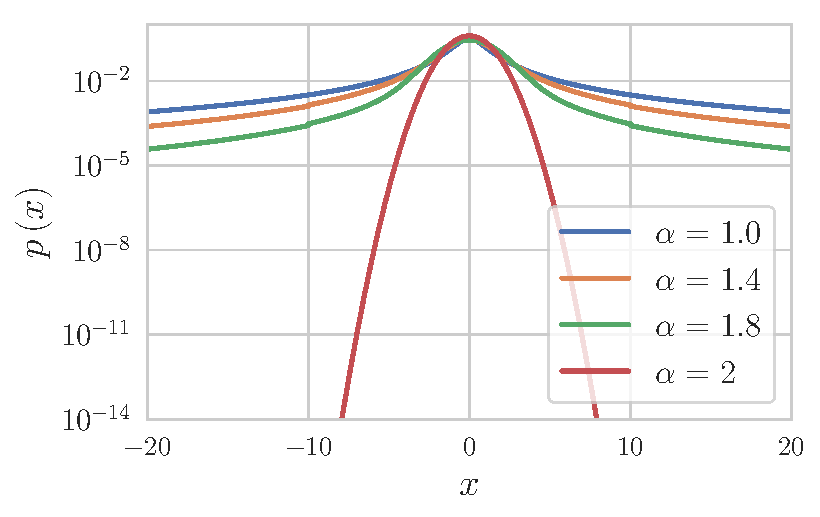
\includegraphics[width=0.8\columnwidth]{distribution_alpha-stable}\caption{$S\alpha S_{c}^{1}$ density probability functions in the real case
with~$\sigma=1$\label{fig:alpha-stable distribution}}
\end{figure}
An isotropic \textcolor{black}{(circular)} symmetric $\alpha$-stable
scalar random variable $x\sim S\alpha S_{c}^{1}\left(\sigma_{x}\right)$
can be defined by its characteristic function (chf.)~$\varphi_{x}:u\in\mathbb{K}\mapsto\mathbb{E}\left(\exp\left(i\Re\left(u^{\star}x\right)\right)\right)$
as follows:
\[
\forall u\in\mathbb{K},\:\varphi_{x}\left(u\right)=\exp\left(-\left|u\right|^{\alpha}\sigma_{x}^{\alpha}\right)
\]
where $\sigma_{x}$ is called a \emph{scale factor}. The real number
$\alpha\in\left(0,2\right]$ is called the\emph{ characteristic exponent}
and defines the heaviness of the tails in a stable distribution: the
smaller~$\alpha$, the heavier the tails. Examples of probability
density functions (pdf.) for such scalar random variables are represented
in the real case in Fig.~\ref{fig:alpha-stable distribution}. It
is remarkable that such a pdf. is not available in closed-form in
general, but only in some particular cases, like the Cauchy~$\left(\alpha=1\right)$
and Gaussian $\left(\alpha=2\right)$ distributions.

\begin{comment}
Avant d'introduire le cas vectoriel, il faudrait d'abord introduire
le cas scalaire, plus simple, et que tu mentionnes plus tard dans
l'article, sans l'avoir d�fini et sans avoir d�fini la notion de ``scale
factor''.
\end{comment}


\subsection{$\alpha$-stable random vectors}

In this paper, we limit our attention to symmetric $\alpha-$stable
random vectors, i.e. $\alpha$-stable random vectors $\boldsymbol{x}$
such that $\boldsymbol{x}$ and $-\boldsymbol{x}$ have the same distribution,
defined as in~(\citet{samoradnitsky1994stable}):
\begin{defn}
\emph{\label{def:spatial_density}Let~$\boldsymbol{x}$ be a random
vector in~$\mathbb{K}^{K}$ associated to its characteristic function~$\varphi_{\boldsymbol{x}}:\boldsymbol{u}\in\mathbb{K}^{K}\mapsto\mathbb{E}\left(\exp\left(i\Re\left\langle \boldsymbol{u},\boldsymbol{x}\right\rangle \right)\right)$.
A symmetric isotropic $\alpha$-stable distribution with $\alpha\in\left(0,2\right)$
is fully described by the unique representation:}

\emph{
\begin{equation}
\forall\boldsymbol{u}\in\mathbb{K}^{K},\:\varphi_{\boldsymbol{x}}\left(\boldsymbol{u}\right)=\exp\left(-\int_{\boldsymbol{\theta}\in\mathcal{S}^{K}}\left|\left\langle \boldsymbol{u},\boldsymbol{\theta}\right\rangle \right|^{\alpha}\Gamma_{\boldsymbol{x}}\left(d\boldsymbol{\theta}\right)\right),\label{eq:spectral_measure}
\end{equation}
where $\Gamma_{\boldsymbol{x}}$ is a symmetric measure on the sphere~$\mathcal{S}^{K}$
called the }spatial density\emph{}\footnote{See Footnote~\vref{fn:spatial_not_spectral}\emph{.}}\emph{.
Henceforth, we note $\boldsymbol{x}\sim S\alpha S_{c}^{K}\left(\Gamma_{\boldsymbol{x}}\right)$
whenever~$\boldsymbol{x}$ follows a symmetric $\alpha$-stable distribution
with }spatial density\emph{~$\Gamma_{\boldsymbol{x}}$.}\footnote{$\Gamma_{\boldsymbol{x}}$ is a symmetric measure on $\mathcal{S}^{K}$
in the sense that for any continuous function $f$ defined on $\mathcal{S}^{K}$
and for any $z\in\mathbb{K}$ such that $\left|z\right|=1$, we have
$\int_{\boldsymbol{\theta}\in\mathcal{S}^{K}}f\left(\boldsymbol{\theta}\right)\Gamma_{\boldsymbol{x}}\left(zd\boldsymbol{\theta}\right)=\int_{\boldsymbol{\theta}\in\mathcal{S}^{K}}f\left(\boldsymbol{\theta}\right)\Gamma_{\boldsymbol{x}}\left(d\boldsymbol{\theta}\right)$.}
\end{defn}
\begin{rem}
A symmetric $\alpha-$stable vector $\boldsymbol{x}\sim S\alpha S_{c}^{K}\left(\Gamma_{\boldsymbol{x}}\right)$
belongs to a larger class: the \emph{elliptically multivariate contoured}
(EMC) distribution~(\citet{cambanis1981theory}). In many cases,
the sum of EMC vectors $\boldsymbol{x},\boldsymbol{y}$, respectively
associated to the so-called scatter matrices $\boldsymbol{R}_{\boldsymbol{x}}$
and $\boldsymbol{R}_{\boldsymbol{y}}$, is still an EMC vector. However,
the parameter $\boldsymbol{R}_{\boldsymbol{x}+\boldsymbol{y}}$ called
\emph{scatter matrix }of the mix is usually not equal to $\boldsymbol{R}_{\boldsymbol{x}}+\boldsymbol{R}_{\boldsymbol{y}}$.
In the $\alpha-$stable case, Definition \ref{def:spatial_density}
ensures that the \emph{spatial density} of the mix $\Gamma_{\boldsymbol{x}+\boldsymbol{y}}$
is equal to $\Gamma_{\boldsymbol{x}}+\Gamma_{\boldsymbol{y}}$.
\end{rem}
We highlight the fact that the Gaussian $\left(\alpha=2\right)$ case
is omitted in Definition~\ref{def:spatial_density}, because the
representation~\eqref{eq:spectral_measure} is not unique in that
case.

\subsection{Spatial spectrum and spatial representation}

In this section, we show how the spatial density~$\Gamma_{\boldsymbol{x}}$,
featured in Definition~\ref{eq:spectral_measure}, of a symmetric
$\alpha$ -stable distribution can be understood through a so-called\emph{
spatial representation}, which is central to the filtering methods
we propose later in Sections~\ref{sec:Multivariate-Filtering-Through-1}
and~\ref{sec:Multivariate-Filtering-Through}.

Let~$\mathcal{X}$ be an independently scattered $\alpha$-stable
random measure on~$\mathcal{S}^{K}$, with control measure~$\Gamma_{\boldsymbol{x}}$~(\citet{samoradnitsky1994stable}).
This means that:
\begin{enumerate}
\item for any Borelian set $A\subset\mathcal{B}\left(\mathcal{S}^{K}\right)$,
the scalar random variable $\mathcal{X}\left(A\right)\in\mathbb{K}$
is distributed as~$\mathcal{X}\left(A\right)\sim S\alpha S_{c}\left(\Gamma_{\boldsymbol{x}}\left(A\right)\right)$,
\item $\mathcal{X}\left(A\right)$ is independent from $\mathcal{X}\left(B\right)$
whenever~$A\cap B=\emptyset$ for any two Borelian subsets~$A$
and $B\subset\mathcal{B}\left(\mathcal{S}^{K}\right)$.
\end{enumerate}
We call~$\mathcal{X}$ the\emph{ spatial spectrum} of the distribution
$S\alpha S_{c}^{K}\left(\Gamma_{\boldsymbol{x}}\right)$.
\begin{rem}
In (\citet{ma1995parameter}), the \emph{$\alpha-$spectrum} terminology
is used in a different way as the \emph{spatial spectrum. }It describes
the so-called covariation (see Section \ref{subsec:Covariation-between-stable}
for further details) between the input single-channel signal and the
output single-channel signal.We have the following first result:
\end{rem}
\begin{thm}
\label{thm:spatial_representation}Let $\boldsymbol{x}\sim S\alpha S_{c}^{K}\left(\Gamma_{\boldsymbol{x}}\right)$,
with spatial density~$\Gamma_{\boldsymbol{x}}$. Then~$\boldsymbol{x}$
admits the following\textbf{ }\emph{spatial representation}:

\begin{equation}
\boldsymbol{x}\overset{d}{=}\int_{\boldsymbol{\theta}\in\mathcal{S}^{K}}\boldsymbol{\theta}\mathcal{X}\left(d\boldsymbol{\theta}\right),\label{eq:spatial_representation}
\end{equation}
where~$\overset{d}{=}$ means ``equal in distribution'' and~$\mathcal{X}$
is the \emph{spatial spectrum} with control measure~$\Gamma_{\boldsymbol{x}}$.
\end{thm}
The proof of this result is given in Appendix~1. The representation
theorem means that an $S\alpha S_{c}^{K}$ random vector is distributed
as the sum of infinitely many contributions, coming from all directions~$\boldsymbol{\theta}\in\mathcal{S}^{K}$
on the sphere. $\Gamma_{\boldsymbol{x}}\left(d\boldsymbol{\theta}\right)$
may thus be interpreted as the \emph{scale factor} of the contributions
pointing in direction~$\boldsymbol{\theta}$. Very interestingly,
the spatial representation in Theorem~\ref{thm:spatial_representation}
provides a straightforward way to generate samples from $S\alpha S_{c}^{K}\left(\Gamma_{\boldsymbol{x}}\right)$
random vectors: first, generate the spatial spectrum $\mathcal{X}$,
and then use~\eqref{eq:spatial_representation} to construct the
$S\alpha S_{c}^{K}$ random vector $\boldsymbol{x}$. The method is
summarized in Algorithm~\ref{alg:alg-synthesis}.

The integration over the real or complex sphere, appearing in~\eqref{eq:spatial_representation},
is replaced by finite sums. This is done by simply constructing a
regular partition~$\Theta$ of the sphere~$\mathcal{S}^{K}$, and
substituting the integration by the corresponding sum carried over
the~$\Theta_{p}$'s. Let~$f$ be a function defined on the hypersphere
and~$M$ be a measure on the sphere. For~$P$ large enough, the
approximation goes as:
\begin{equation}
\int_{\mathcal{S}^{K}}\boldsymbol{\theta}f\left(\boldsymbol{\theta}\right)M\left(d\boldsymbol{\theta}\right)\approx\sum_{p}\boldsymbol{\theta}_{p}f\left(\boldsymbol{\theta}_{p}\right)M\left(\Theta_{p}\right),\label{eq:riemann_approx-1}
\end{equation}
where~$M\left(\Theta_{p}\right)$ may further be approximated as~$m\left(\boldsymbol{\theta}_{p}\right)\Delta_{\Theta}$
(where $\Delta_{\Theta}$ is the Lebesgue measure of $\Theta_{p}$),
whenever~$M$ is dominated by the Lebesgue measure and thus equal
to~$M\left(d\boldsymbol{\theta}\right)=m\left(\boldsymbol{\theta}\right)d\boldsymbol{\theta}$
for some measurable function~$m$.

\begin{algorithm}[H]
\begin{enumerate}
\item \textbf{Input}
\begin{itemize}
\item Number~$N$ of desired realizations
\item Partition~$\Theta=\left\{ \Theta_{1},\dots,\Theta_{P}\right\} $
of~$\mathcal{S}^{K}$ as described in Section~\ref{subsec:Notations}
\item Characteristic exponent~$\alpha\in\left(0,2\right)$
\item Spatial density~$\Gamma_{\boldsymbol{x}}$
\end{itemize}
\item \textbf{Spatial spectrum generation}\\
\textbf{$\forall n,p,\,\mathcal{X}_{np}\sim S\alpha S_{c}\left(\Gamma_{\boldsymbol{x}}\left(\Theta_{p}\right)\right)$
}where $\Gamma_{\boldsymbol{x}}\left(\Theta_{p}\right)$ is the restriction
of $\Gamma_{\boldsymbol{x}}$ to the set $\Theta_{p}$ up to renormalization.\vspace{0.09cm}
\item \textbf{Synthesis} $\forall n,x_{n}\leftarrow\sum_{p}\boldsymbol{\theta}_{p}\mathcal{X}_{np}$
\end{enumerate}
\caption{Sampling of $S\alpha S_{c}^{K}\left(\Gamma_{\boldsymbol{x}}\right)$
random vectors through their spatial representation\label{alg:alg-synthesis}.}
\end{algorithm}

Given our model for $\alpha$-stable vectors, we now discuss the distribution
of mixtures of such random vectors.

\subsection{Mixtures of $\alpha$-stable random vectors\label{subsec:Mixtures-of-alpha-stable}}

\begin{figure}[h]
\centering{}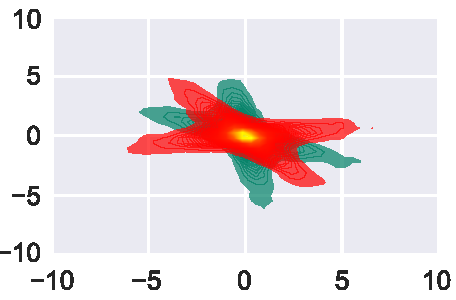
\includegraphics[width=0.5\columnwidth]{double_VonMises}~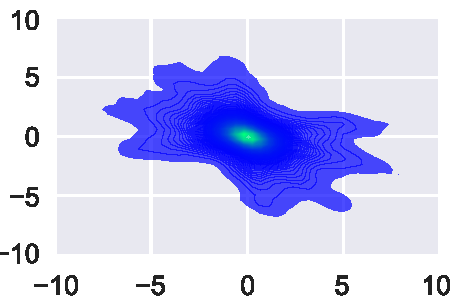
\includegraphics[width=0.5\columnwidth]{double_VonMises(melange)}\caption{\label{fig:Example-of-spatial}Spatial densities in the real case
with $K=2$. \textbf{On the left}, density plots of~$\boldsymbol{y}_{1}\sim S\alpha S_{c}^{K}\left(\Gamma_{1}\right)$
(in green) and~$\boldsymbol{y}_{2}\sim S\alpha S_{c}^{K}\left(\Gamma_{2}\right)$
(in red), where the maxima of~$\Gamma_{1}$ and~$\Gamma_{2}$ are
reached for~$\left\{ \frac{5\pi}{8},\frac{5\pi}{8}+\frac{\pi}{3}\right\} $
and~$\left\{ \frac{5\pi}{8}+\frac{\pi}{6},\frac{5\pi}{8}+\frac{\pi}{2}\right\} $.
These plots show the influence of the spatial density on the dependence
patterns between covariates. \textbf{On the right}, a density plot
for the mixture~$\boldsymbol{x}=\boldsymbol{y}_{1}+\boldsymbol{y}_{2}$
shows the additive property of spatial densities.}
\end{figure}

In the filtering and signal processing literature, it is common to
assume that the observed vector~$\boldsymbol{x}\in\mathbb{K}^{K}$
is the sum of~$J$ components~$\boldsymbol{y}_{j}\in\mathbb{K}^{K}$
that we want to recover. Here, we take each component~$\boldsymbol{y}_{j}\sim S\alpha S_{c}^{K}\left(\Gamma_{j}\right)$
as described above, with its own spatial density~$\Gamma_{j}$:
\begin{equation}
\begin{cases}
\boldsymbol{x}=\sum_{j=1}^{J}\boldsymbol{y}_{j}\\
\forall j,\,\boldsymbol{y}_{j}\sim S\alpha S_{c}^{K}\left(\Gamma_{j}\right).
\end{cases}\label{eq:image_sources_model}
\end{equation}
Because~$\boldsymbol{x}$ is the sum of $\alpha$-stable vectors,
then~$\boldsymbol{x}$ itself follows an $\alpha$-stable distribution,
with the following spatial density:

\[
\begin{cases}
\boldsymbol{x}\sim S\alpha S_{c}^{K}\left(\Gamma_{\boldsymbol{x}}\right)\\
\Gamma_{\boldsymbol{x}}=\sum_{j}\Gamma_{j}.
\end{cases}
\]
By invoking the spatial representation Theorem~\ref{thm:spatial_representation}
on each latent vector~$\boldsymbol{y}_{j}$, we get: $\forall j,\:\boldsymbol{y}_{j}\overset{d}{=}\int_{\boldsymbol{\theta}\in\mathcal{S}^{K}}\boldsymbol{\theta}\mathcal{Y}_{j}\left(d\boldsymbol{\theta}\right)$,
where~$\mathcal{Y}_{j}$ denotes the spatial spectrum of~$\boldsymbol{y}_{j}$.
Moreover, $\mathcal{X}\triangleq\sum_{j}\mathcal{Y}_{j}$ also defines
a spatial spectrum associated to~$\boldsymbol{x}$. Informally, it
simply means that~$\boldsymbol{x}$ is also the sum of infinitely
many contributions~$\mathcal{X}\left(d\boldsymbol{\theta}\right)$,
coming from all directions~$\boldsymbol{\theta}\in\mathcal{S}^{K}$
on the sphere, each one of them being in turn the sum of the contributions~$\mathcal{Y}_{j}\left(d\boldsymbol{\theta}\right)$
for all components that come from this particular direction. An illustration
of the relationships between the spatial densities~$\Gamma_{\boldsymbol{x}},\Gamma_{j}$
is given in Fig.~\ref{fig:Example-of-spatial}.

The next two sections make different uses of this spatial representation
to devise\emph{ filters}, which aim at estimating the latent vectors~$\boldsymbol{y}_{j}$
given $\boldsymbol{x}$, provided the spatial densities~$\Gamma_{j}$,
which are parameters, are \emph{known}. This allows us to dissociate
the actual filtering problem from the question of estimating signal
parameters. This strategy is for instance classical in the literature
focusing on Wiener-based filter design~(\citet{wiener1949extrapolation,duong_TSALP2010}).

\section{Spatial spectrum filter (SSF) \label{sec:Multivariate-Filtering-Through-1}}

Our objective is to estimate each latent vector~$\boldsymbol{y}_{j}$,
such that~$\sum\boldsymbol{y}_{j}=\boldsymbol{x}$. The strategy
we discuss here proceeds in two steps. Firstly, we estimate the spatial
spectrum~$\mathcal{X}$ of the mixture, as described in Section~\ref{subsec:Isotropic-random-measure}.
Secondly, this estimate is used to reconstruct the desired latent
vectors~$\boldsymbol{y}_{j}$, as detailed in Section~\ref{subsec:Multivariate-signal-reconstructi}.

\subsection{Spatial spectrum estimation~\label{subsec:Isotropic-random-measure}}

We assume that the observation~$\boldsymbol{x}\sim S\alpha S_{c}^{K}\left(\Gamma_{\boldsymbol{x}}\right)$
and its spatial density $\Gamma_{x}$ are known. The first step in
the filter we discuss here is to estimate the spatial spectrum~$\mathcal{X}$.
For this purpose, we choose the \emph{a posteriori} expectation $\widehat{\mathcal{X}}\left(d\boldsymbol{\theta}\right)$
of $\mathcal{X}\left(d\boldsymbol{\theta}\right)$ given $\boldsymbol{x}$,
defined in the following sense: for any continuous function~$\psi$
on $\mathcal{S}^{K}$, satisfying $\int_{\boldsymbol{\theta}\in S^{K}}\left|\psi\left(\boldsymbol{\theta}\right)\right|^{\alpha}\Gamma_{\boldsymbol{x}}\left(d\boldsymbol{\theta}\right)<+\infty$,
we have:

\begin{equation}
\mathbb{E}\left[\int_{\boldsymbol{\theta}\in\mathcal{S}^{K}}\text{\ensuremath{\psi\left(\boldsymbol{\theta}\right)}}\mathcal{X}\left(d\boldsymbol{\theta}\right)\mid\boldsymbol{x}\right]=\int_{\boldsymbol{\theta}\in\mathcal{S}^{K}}\psi\left(\boldsymbol{\theta}\right)\widehat{\mathcal{X}}\left(d\boldsymbol{\theta}\right).\label{eq:estimator_criterion}
\end{equation}
Note that it is such that $\int_{\boldsymbol{\theta}\in\mathcal{S}^{K}}\boldsymbol{\theta}\widehat{\mathcal{X}}\left(d\boldsymbol{\theta}\right)=\boldsymbol{x}$.
It turns out that in the particular case of an~$S\alpha S_{c}^{K}\left(\Gamma_{\boldsymbol{x}}\right)$
observation~$\boldsymbol{x}$, $\widehat{\mathcal{X}}\left(d\boldsymbol{\theta}\right)$
has the following form:
\begin{prop}
\label{prop:spatial_spectrum_form1}Under the previous assumptions,~$\widehat{\mathcal{X}}\left(d\boldsymbol{\theta}\right)$
can be rewritten as:
\begin{equation}
\widehat{\mathcal{X}}\left(d\boldsymbol{\theta}\right)=\gx\left(\boldsymbol{x},\boldsymbol{\theta}\right)\Gamma_{\boldsymbol{x}}\left(d\boldsymbol{\theta}\right)\quad\text{a.s.}\label{eq:estimator_form}
\end{equation}
with:

\begin{equation}
\forall\boldsymbol{\theta}\in\mathcal{S}^{K},\:\gx\left(\boldsymbol{x},\boldsymbol{\theta}\right)=\frac{N\left(\boldsymbol{x},\boldsymbol{\theta}\right)}{D\left(\boldsymbol{x}\right)},\label{eq:estimation_g_x_theta}
\end{equation}
where

\begin{equation}
N\left(\boldsymbol{x},\boldsymbol{\theta}\right)=\alpha i\int_{\boldsymbol{u}\in\mathbb{K}^{K}}\text{\ensuremath{\left\langle \boldsymbol{\theta},\boldsymbol{u}\right\rangle }}{}^{\left\langle \alpha-1\right\rangle }\varphi_{\boldsymbol{x}}\left(\boldsymbol{u}\right)\,e^{-i\Re\left(\left\langle \boldsymbol{u},\boldsymbol{x}\right\rangle \right)}d\boldsymbol{u}\label{eq:N}
\end{equation}
and
\begin{equation}
D\left(\boldsymbol{x}\right)=\int_{\boldsymbol{u}\in\mathbb{K}^{K}}\varphi_{\boldsymbol{x}}\left(\boldsymbol{u}\right)\,e^{-i\Re\left(\left\langle \boldsymbol{u},\boldsymbol{x}\right\rangle \right)}d\boldsymbol{u}.\label{eq:D}
\end{equation}

If~$\alpha>1$, the density~$\gx\left(\boldsymbol{x},\boldsymbol{\theta}\right)$
is a continuous map on~$\mathcal{S}^{K}$, and hence the measure~$\widehat{\mathcal{X}}\left(d\boldsymbol{\theta}\right)$
is dominated by~$\Gamma_{\boldsymbol{x}}\left(d\boldsymbol{\theta}\right)$.
\end{prop}
Proposition~\ref{prop:spatial_spectrum_form1} is proved in Appendix~2.

Although~$\gx\left(\boldsymbol{x},\boldsymbol{\theta}\right)$ has
the closed-form expression \eqref{eq:estimation_g_x_theta}, its computation
is not straightforward because it requires two integrations over~$\mathbb{K}^{K}$.
Let $I_{\boldsymbol{x}}\left(\boldsymbol{u}\right)\triangleq-\ln\left(\varphi_{\boldsymbol{x}}\left(\boldsymbol{u}\right)\right)$
be the Levy exponent of~$\boldsymbol{x}$~(\citet{unser2014introduction}).
From~\eqref{eq:spectral_measure}, it is given by: $I_{\boldsymbol{x}}\left(\boldsymbol{u}\right)=\int_{\boldsymbol{\theta}\in\mathcal{S}^{K}}\left|\left\langle \boldsymbol{u},\boldsymbol{\theta}\right\rangle \right|^{\alpha}\Gamma_{\boldsymbol{x}}\left(d\boldsymbol{\theta}\right)$.
We have the following result, with proofs given in Appendix~2:
\begin{prop}
\label{prop:numerator_calculation}Let $\beta=1$ if $\mathbb{K}=\mathbb{R}$,
or $\beta=$2 if $\mathbb{K}=\mathbb{C}.$ Then \eqref{eq:N} is equivalent
to

\begin{equation}
N\left(\boldsymbol{x},\boldsymbol{\theta}\right)=\int_{\boldsymbol{\theta}'\in\mathcal{S}^{K}}\frac{\left\langle \boldsymbol{\theta},\boldsymbol{\theta'}\right\rangle {}^{\left\langle \alpha-1\right\rangle }\left\langle \boldsymbol{\theta'},\boldsymbol{x}\right\rangle }{I_{\boldsymbol{x}}\left(\boldsymbol{\theta'}\right){}^{\frac{\beta K+\alpha}{\alpha}}}\eta\left(\frac{\left|\left\langle \boldsymbol{\theta'},\boldsymbol{x}\right\rangle \right|^{2}}{I_{\boldsymbol{x}}\left(\boldsymbol{\theta'}\right){}^{\frac{2}{\alpha}}}\right)d\boldsymbol{\theta'},\label{eq:numerator}
\end{equation}
where:
\begin{equation}
\eta\left(\rho\right)=\sum_{n=0}^{+\infty}\frac{\left(-1\right){}^{n}f_{\Gamma}\left(\frac{2n+\beta K+\alpha}{\alpha}\right)}{2^{2n+1}n!\left(n+1\right)!}\rho^{n}.\label{eq:eta}
\end{equation}
with $f_{\Gamma}$ the Gamma function. In the same way, \eqref{eq:D}
is equivalent to

\begin{equation}
D\left(\boldsymbol{x}\right)=\frac{\left\Vert \int_{\mathcal{S}^{K}}\boldsymbol{\theta}N\left(\boldsymbol{x},\boldsymbol{\theta}\right)\Gamma_{x}\left(d\boldsymbol{\theta}\right)\right\Vert _{1}}{\left\Vert \boldsymbol{x}\right\Vert _{1}}.\label{eq:Denominator}
\end{equation}
\end{prop}
Proposition~\ref{prop:numerator_calculation} is proved in Appendix~2.

Note that in \eqref{eq:Denominator}, any norm could be picked for
the computation and yield the same result. The~$\ell_{1}-$norm~$\left\Vert .\right\Vert {}_{1}$
turns out to be a good compromise between computational cost and numerical
stability.

Equations~\eqref{eq:numerator} and~\eqref{eq:Denominator} in Proposition~\ref{prop:numerator_calculation}
provide an estimator of~$\gx$, which is computationally tractable
via integrations on the compact set $\mathcal{S}^{K}$, as opposed
to~\eqref{eq:estimation_g_x_theta} that requires integration over
$\mathbb{K}^{K}$.

The quantity~$\eta\left(\rho\right)$ is a power series with an infinite
radius of convergence when~$\alpha>1$. It is a smooth function of~$\rho$
and independent of the data and the model parameters. It can hence
be computed beforehand.

The main computational burden for this method lies in the computation
of the alternating power series~$\eta$ in~\eqref{eq:eta}. It converges
slowly and goes through extreme values, requiring a fairly large numerical
precision in practice. However, there are some cases where a closed-form
expression is available, for instance when~$\alpha=2,\,K=2$, $\beta=2$,
where~$\eta\left(\rho\right)=\frac{1}{16}\left(\rho^{2}-20\rho+64\right)e^{-\rho/4}$.
Inspired by this result, we decided to approximate~$\eta$ in all
cases as:\vspace{-0.25cm}

\begin{equation}
\eta\left(\rho\right)\approx\widehat{\eta}\left(\rho\right)=\left(a\rho^{2}+b\rho+c\right)e^{-d\rho}\label{eq:eta_fitting}
\end{equation}
where~$a,b,c,d\in\mathbb{R}$ are model parameters. Using such a
parameterized version allows us to avoid the on-demand time-consuming
evaluations of~$\eta$. We estimated the parameters that minimize
the mean-square-error (MSE)~$\left\Vert \eta-\hat{\eta}\right\Vert _{2}^{2}$.
We highlight that both the choice of this parametric model \eqref{eq:eta_fitting}
and the choice of the MSE criterion are driven by ad-hoc considerations,
indeed, there is no theoretical result we are aware of that would
justify the convergence of the power series to an exponential function.
However, the plots for~$\eta$ and~$\hat{\eta}$ for $\beta=1$
are displayed in Fig.~\ref{fig:Curve-fitting_eta}, and the error
of fit for~$\eta$ for $\beta=2$ as a function of~$\alpha$ is
displayed in Fig.~\ref{fig:Curve-fitting_eta-MSE} and quality is
very good. Results were similar in the real and complex cases. $\eta$
was computed for~$50$ regularly spaced values~$\alpha\in\left(1,2\right)$,
and for~$\rho\in\left(0,10\right)$, because~$\rho$ only has positive
values in~\eqref{eq:numerator}. For getting a suitable convergence,~$\eta$
was calculated up to order~$10^{5}$.

\begin{figure}[H]
\begin{centering}
\subfigure[$\eta$ and~$\hat{\eta}$ for~$\alpha=1.3$ and $\beta=1$
.\label{fig:Curve-fitting_eta}]{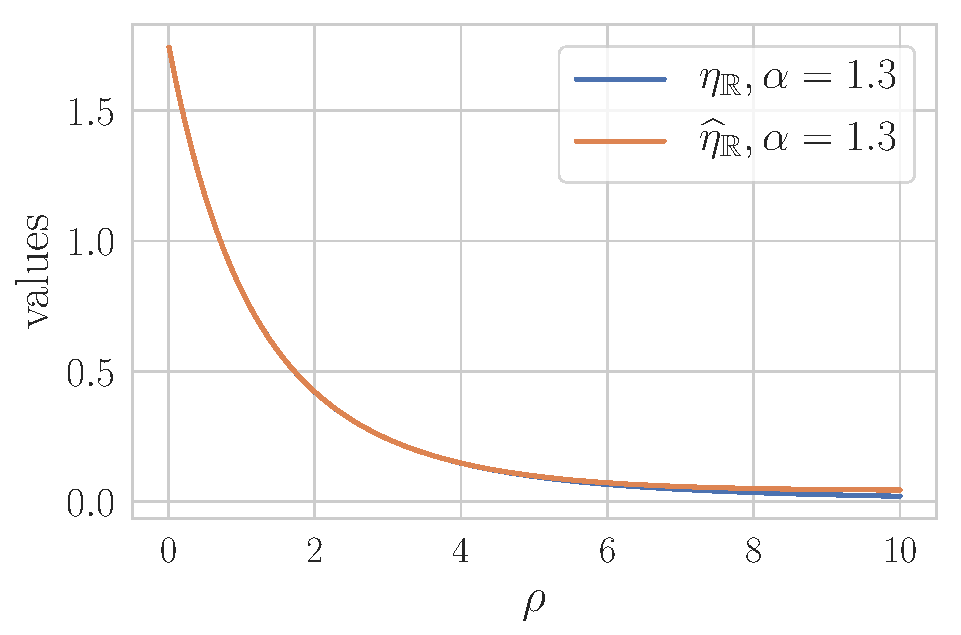
\includegraphics[width=0.6\columnwidth]{eta_example}}\\
\hspace{-0.2cm}\subfigure[MSE as a function of~$\alpha.$\label{fig:Curve-fitting_eta-MSE}]{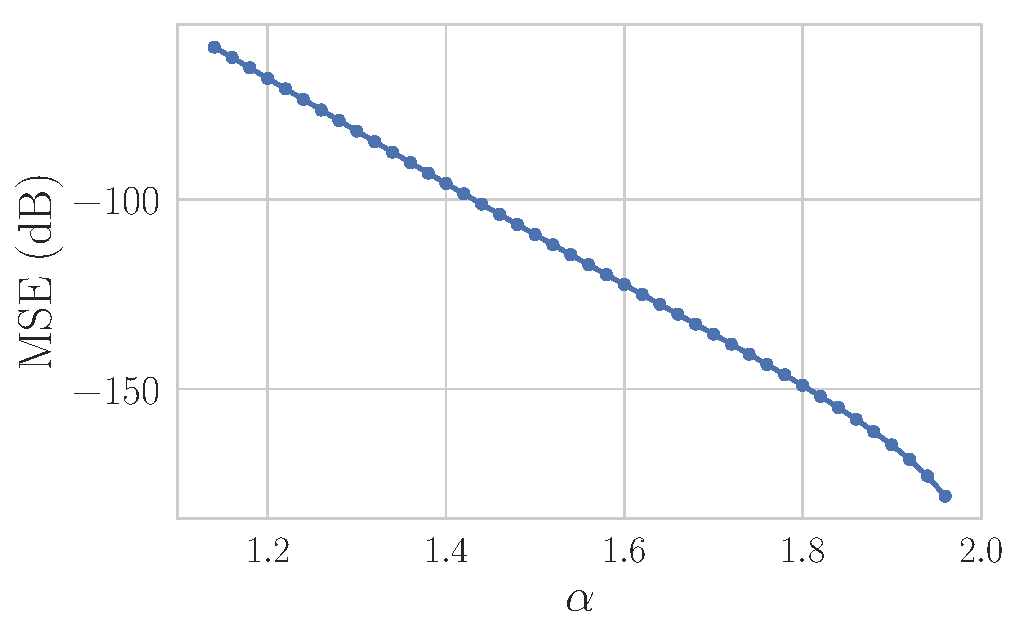
\includegraphics[width=0.63\columnwidth]{eta_estimation}}
\par\end{centering}
\centering{}\caption{Performance of a parametric fit~$\hat{\eta}$ for~$\eta$ in~\eqref{eq:eta}
.}
\end{figure}

\vspace{-0.5cm}

\subsection{Signal reconstruction\label{subsec:Multivariate-signal-reconstructi}}

Once the spatial spectrum $\mathcal{X}\left(d\boldsymbol{\theta}\right)$
of the observation is estimated, or equivalently~$\gx\left(\boldsymbol{x},\boldsymbol{\theta}\right)$
is computed through~\eqref{eq:estimation_g_x_theta}, \eqref{eq:numerator}
and~\eqref{eq:Denominator}, our next step is to construct an estimate
for the components~$\boldsymbol{y}_{j}$ of interest. We pick the
\emph{a posteriori} expectation:~$\widehat{\boldsymbol{y}}_{j}\triangleq\mathbb{E}\left[\boldsymbol{y}_{j}\mid\boldsymbol{x}\right]$,
which is given as follows:
\begin{thm}
\label{thm:source_reconstruction}Let~$\boldsymbol{x}$ be the sum
of $S\alpha S_{c}^{K}$ random vectors~$\boldsymbol{y}_{j}\sim S\alpha S_{c}^{K}\left(\Gamma_{j}\right)$,
each with known spatial density~$\Gamma_{j}$. Then the \emph{a~posteriori}
expectation of each component~$\boldsymbol{y}_{j}$ given $\boldsymbol{x}$
is:

\begin{equation}
\widehat{\boldsymbol{y}}_{j}\triangleq\mathbb{E}\left[\boldsymbol{y}_{j}\mid\boldsymbol{x}\right]=\int_{\boldsymbol{\theta}\in\mathcal{S}^{K}}\boldsymbol{\theta}\gx\left(\boldsymbol{x},\boldsymbol{\theta}\right)\Gamma_{j}\left(d\boldsymbol{\theta}\right),\label{eq:reconstruction_result}
\end{equation}
where~$\gx$ was defined in~\eqref{eq:estimation_g_x_theta}.
\end{thm}
The proof of this theorem is also in Appendix~2. A summary of this
filtering technique is given in Algorithm~\ref{alg:algorithm}:
\begin{algorithm}[H]
\begin{enumerate}
\item \textbf{Input}
\begin{itemize}
\item Observation~$\boldsymbol{x}$ of size~$K$
\item Regular partition~$\Theta=\left\{ \Theta_{1},\dots,\Theta_{P}\right\} $
of~$\mathcal{S}^{K}$
\item Characteristic exponent~$\alpha\in\left(1,2\right)$
\item spatial densities~$\Gamma_{j}$
\end{itemize}
\item \textbf{Spatial spectrum estimation}
\begin{itemize}
\item Using~$\hat{\eta}$ in~\eqref{eq:eta_fitting}, compute~$\forall p,\,N\left(\boldsymbol{x},\boldsymbol{\theta}_{p}\right)$
in~\eqref{eq:numerator}
\item Compute~$D\left(\boldsymbol{x}\right)$ in~\eqref{eq:Denominator}
\item Compute~$\gx\left(\boldsymbol{x},\boldsymbol{\theta}_{p}\right)=\frac{N\left(\boldsymbol{x},\boldsymbol{\theta}_{p}\right)}{D\left(\boldsymbol{x}\right)}$
\end{itemize}
\item \textbf{Reconstruction:~$\widehat{\boldsymbol{y}}_{j}=\sum_{p}\boldsymbol{\theta}_{p}\gx\left(x,\boldsymbol{\theta}_{p}\right)\Gamma_{j}\left(\Theta_{p}\right)$}
\end{enumerate}
\caption{\textbf{$\alpha-$SSF}: multivariate~$\alpha$-stable filtering through
a spatial spectrum estimation\label{alg:algorithm}.}
\end{algorithm}


\section{Covariation-minimizing filter (CMF)\label{sec:Multivariate-Filtering-Through}}

Despite a relatively simple expression of $\gx$, the estimation technique
in Section~\ref{sec:Multivariate-Filtering-Through-1} is computationally
demanding, due to several numerical integrations. In this section,
the spatial representation in~Theorem \ref{thm:spatial_representation}
will be exploited differently, leading to a faster filtering method.

\subsection{Covariation between stable variables\label{subsec:Covariation-between-stable}}

Many signal processing studies exploit second-order statistics for
the design of digital filters~(\citet{cardoso1998blind,duong_TSALP2010,moussaoui2008decomposition}).
This convenient strategy finds a straightforward probabilistic interpretation
through Gaussian processes~$(\alpha=2$), that are characterized
by their covariance functions. However, this strategy breaks down
for $\alpha$-stable processes with~$\alpha<2$, because the moments
of order~$p\geq\alpha$ are infinite. For this reason, the \emph{covariation}
was introduced\emph{~}(\citet[p. 87]{samoradnitsky1994stable,nikias1995signal})
as a substitute of the covariance, with many similar properties.
\begin{defn}
The covariation between two random variables~$\left(x_{1},x_{2}\right)$,
jointly distributed as: $\left(x_{1},x_{2}\right)\triangleq\boldsymbol{x}\sim S\alpha S_{c}^{2}\left(\Gamma_{\boldsymbol{x}}\right)$
for~$\alpha>1$, is defined as:

\[
\left[x_{1},x_{2}\right]_{\alpha}\triangleq\int_{\boldsymbol{z}=\left(z_{1},z_{2}\right)\in\mathcal{S}^{2}}z_{1}^{\ast}z_{2}^{\left\langle \alpha-1\right\rangle }\Gamma_{\boldsymbol{x}}\left(d\boldsymbol{z}\right).
\]

Moreover, the\emph{ covariation norm~}(\citet[p 95]{samoradnitsky1994stable})
of~$u\sim S\alpha S_{c}^{1}$ is:

\[
\left\Vert u\right\Vert {}_{\alpha}=\left(\left[u,u\right]_{\alpha}\right)^{1/\alpha}.
\]
\end{defn}
\begin{rem}
\label{rem:The-covariation-is}The covariation is always anti-linear
in its left argument. It is also linear in the right argument if and
only if all terms of the linear combination on the right-hand side
are mutually independent: if $\left(x,x_{1},x_{2}\right)$ are jointly
$S\alpha S_{c}^{3}$ with~$x_{1}$ and~$x_{2}$ independent, then
$\left[x,x_{1}+x_{2}\right]_{\alpha}=\left[x,x_{1}\right]_{\alpha}+\left[x,x_{2}\right]_{\alpha}$.
In addition, if~$x_{1}$ and~$x_{2}$ are independent then~$\left[x_{1},x_{2}\right]_{\alpha}=0$,
and if~$x\sim S\alpha S_{c}^{1}\left(\sigma_{x}\right)$,~then~$\left\Vert x\right\Vert _{\alpha}=\sigma_{x}$.
\end{rem}

\subsection{Covariation minimization filtering (CMF) technique\label{subsec:Covariation-filtering-technique}}

Our objective in this section is to build a filter to extract the
component~$\boldsymbol{y}_{j}$ from the mixture~$\boldsymbol{x}$.
Motivated by~(\citet{masry2000alpha}), we seek filtering vectors~$\boldsymbol{w}_{jk}\in\mathbb{K}^{K}$
such that $\widehat{y}_{jk}=\left\langle \boldsymbol{w}_{jk},\boldsymbol{x}\right\rangle $
minimizes the covariation norm~$\left\Vert y_{jk}-\widehat{y}_{jk}\right\Vert {}_{\alpha}^{\alpha}$.
Additionally, we enforce $\ensuremath{\sum_{j}\boldsymbol{w}_{jk}=\boldsymbol{e}_{k}}$
to guarantee perfect reconstruction of the mixture: $\boldsymbol{x}=\sum_{j}\widehat{\boldsymbol{y}}_{j}$.
For each~$k$, this results in the following optimization problem
with linear equality constraints:
\begin{equation}
\begin{array}{cc}
\underset{}{\text{minimize}} & \sum_{j}\left\Vert y_{jk}-\left\langle \boldsymbol{w}_{jk},\boldsymbol{x}\right\rangle \right\Vert _{\alpha}^{\alpha}\,\mathrm{w.r.t.\,}\boldsymbol{w}_{jk}\\
\text{subject to} & \sum_{j}\boldsymbol{w}_{jk}=\boldsymbol{e}_{k}.
\end{array}\label{eq:optimization_problem}
\end{equation}
The constraints and covariation norm have convenient properties. Firstly,
the constraints are linear. Secondly, the criterion is a differentiable
function whose derivative is continuous, and it is convex. Thirdly,
the covariation norm is coercive. By invoking the Karush, Khun and
Tucker theorem~(\citet{boyd2004convex}), this optimization problem
thus has a unique solution.

We apply the spatial representation in Theorem~\ref{thm:spatial_representation}
to get $\boldsymbol{x}\overset{d}{=}\int\boldsymbol{\theta}\mathcal{X}\left(d\boldsymbol{\theta}\right)$
and $\boldsymbol{y}_{j}\overset{d}{=}\int\boldsymbol{\theta}\mathcal{Y}_{j}\left(d\boldsymbol{\theta}\right)$,
with integrations done over~$S^{K}$. The Lagrangian of the problem~\eqref{eq:optimization_problem}
is
\begin{align}
\mathcal{L}\left(\left\{ \boldsymbol{w}_{jk}\right\} _{j},\boldsymbol{\lambda}_{k}\right) & =\sum_{j}\left\Vert y_{jk}-\left\langle \boldsymbol{w}_{jk},\boldsymbol{x}\right\rangle \right\Vert _{\alpha}^{\alpha}\nonumber \\
 & +\alpha\Re\left(\boldsymbol{\lambda}_{k}^{\ast}\left(\sum_{j}\boldsymbol{w}_{jk}-\boldsymbol{e}_{k}\right)\right)\label{eq:Lagrangian}
\end{align}
where the factor $\alpha$ in the second line is introduced to simplify
the following calculations. Now, thanks to properties of the covariation
given in Remark~\ref{rem:The-covariation-is}, the development of~$\left\Vert y_{jk}-\widehat{y}_{jk}\right\Vert {}_{\alpha}^{\alpha}$
for all~$j,k$ yields:{\footnotesize{}}\\
{\footnotesize{}
\begin{align}
 & \left\Vert y_{jk}-\widehat{y}_{jk}\right\Vert {}_{\alpha}^{\alpha}\nonumber \\
= & \left\Vert y_{jk}-\sum_{j'}\left\langle \boldsymbol{w}_{jk},\boldsymbol{y}_{j'}\right\rangle \right\Vert _{\alpha}^{\alpha}\nonumber \\
= & \left\Vert \int\left(\theta_{k}-\left\langle \boldsymbol{w}_{jk},\boldsymbol{\theta}\right\rangle \right)\mathcal{Y}_{j}\left(d\boldsymbol{\theta}\right)\right\Vert _{\alpha}^{\alpha}+\sum_{j'\neq j}\left\Vert \int\left\langle \boldsymbol{w}_{jk},\boldsymbol{\theta}\right\rangle \mathcal{Y}_{j'}\left(d\boldsymbol{\theta}\right)\right\Vert _{\alpha}^{\alpha}\nonumber \\
= & \int\left|\theta_{k}-\left\langle \boldsymbol{w}_{jk},\boldsymbol{\theta}\right\rangle \right|^{\alpha}\Gamma_{j}\left(d\boldsymbol{\theta}\right)+\sum_{j'\neq j}\int\left|\left\langle \boldsymbol{w}_{jk},\boldsymbol{\theta}\right\rangle \right|^{\alpha}\Gamma_{j'}\left(d\boldsymbol{\theta}\right)\nonumber \\
= & \int\left(\left|\theta_{k}-\left\langle \boldsymbol{w}_{jk},\boldsymbol{\theta}\right\rangle \right|^{\alpha}-\left|\left\langle \boldsymbol{w}_{jk},\boldsymbol{\theta}\right\rangle \right|^{\alpha}\right)\Gamma_{j}\left(d\boldsymbol{\theta}\right)+\int\left|\left\langle \boldsymbol{w}_{jk},\boldsymbol{\theta}\right\rangle \right|^{\alpha}\Gamma_{x}(d\boldsymbol{\theta}).\label{eq:spatial_decomposition_variation_norm}
\end{align}
}{\footnotesize\par}

By substituting~\eqref{eq:spatial_decomposition_variation_norm}
in~\eqref{eq:Lagrangian}, and by zeroing the gradient of~$\mathcal{L}$
w.r.t.~$\boldsymbol{w}_{jk}$, we get for all~$j$:{\small{}
\begin{align}
\boldsymbol{\lambda}_{k}= & \int\boldsymbol{\theta}\left(\left(\theta_{k}^{\ast}-\left\langle \boldsymbol{\theta},\boldsymbol{w}_{jk}\right\rangle \right)^{\left\langle \alpha-1\right\rangle }+\left\langle \boldsymbol{\theta},\boldsymbol{w}_{jk}\right\rangle {}^{\left\langle \alpha-1\right\rangle }\right)\Gamma_{j}\left(d\boldsymbol{\theta}\right)\nonumber \\
 & -\int\boldsymbol{\theta}\left\langle \boldsymbol{\theta},\boldsymbol{w}_{jk}\right\rangle {}^{\left\langle \alpha-1\right\rangle }\Gamma_{x}\left(d\boldsymbol{\theta}\right).\label{eq:grad_lagrangian}
\end{align}
}{\small\par}

By noting that $z^{\left\langle \alpha-1\right\rangle }=\frac{z}{|z|^{2-\alpha}},$~\eqref{eq:grad_lagrangian}
can be written as:

\begin{equation}
\boldsymbol{\lambda}_{k}=-\boldsymbol{P}_{jk}\boldsymbol{w}_{jk}+\boldsymbol{r}_{jk},\label{eq:dev_grad}
\end{equation}
where the $K\times K$ matrix~$\boldsymbol{R}_{jk}$ and the vector
$\boldsymbol{r}_{jk}\in\mathbb{K}^{K}$ are defined as:

{\small{}
\begin{alignat}{1}
\boldsymbol{P}_{jk}= & \int\left(\frac{\boldsymbol{\theta}\boldsymbol{\theta}^{\star}}{\left|\theta_{k}-\left\langle \boldsymbol{w}_{jk},\boldsymbol{\theta}\right\rangle \right|^{2-\alpha}}-\frac{\boldsymbol{\theta}\boldsymbol{\theta}^{\star}}{\left|\left\langle \boldsymbol{w}_{jk},\boldsymbol{\theta}\right\rangle \right|^{2-\alpha}}\right)\Gamma_{j}\left(d\boldsymbol{\theta}\right)\nonumber \\
 & +\int\frac{\boldsymbol{\theta}\boldsymbol{\theta}^{\star}}{\left|\left\langle \boldsymbol{w}_{jk},\boldsymbol{\theta}\right\rangle \right|^{2-\alpha}}\Gamma_{x}\left(d\boldsymbol{\theta}\right).\label{eq:Spatial_covariation_matrix}\\
\boldsymbol{r}_{jk}= & \int\frac{\boldsymbol{\theta}\theta_{k}^{\star}}{\left|\theta_{k}-\left\langle \boldsymbol{w}_{jk},\boldsymbol{\theta}\right\rangle \right|^{2-\alpha}}\Gamma_{j}\left(d\boldsymbol{\theta}\right).\label{eq:cov_vector}
\end{alignat}
}Therefore $\boldsymbol{w}_{jk}$ is a fixed point of the following
equation:

\begin{equation}
\boldsymbol{w}_{jk}=\boldsymbol{P}_{jk}^{-1}\left(\boldsymbol{r}_{jk}-\boldsymbol{\lambda}_{k}\right).\label{eq:w_j,k iteration}
\end{equation}
A sum over~$j$ in~\eqref{eq:w_j,k iteration} leads to:
\begin{equation}
\boldsymbol{\lambda}_{k}=\left(\sum_{j}\boldsymbol{P}_{jk}^{-1}\right)^{-1}\left(\left(\sum_{j}\boldsymbol{P}_{jk}^{-1}\boldsymbol{r}_{jk}\right)-\boldsymbol{e}_{k}\right).\label{eq:lambda_update}
\end{equation}

Putting together the above results, we propose to design the filters
$\boldsymbol{w}_{jk}$ based on a fixed-point approach where~$\boldsymbol{P}_{jk}$
in~\eqref{eq:Spatial_covariation_matrix}, $\boldsymbol{w}_{jk}$
in~\eqref{eq:w_j,k iteration} and $\boldsymbol{\lambda}_{k}$~in~\eqref{eq:lambda_update}
are updated in turn. This is summarized in Algorithm~\ref{alg:MASCOT}.
The integrals are replaced by a discrete sum as in~\eqref{eq:riemann_approx-1}.

\begin{algorithm}[H]
\begin{enumerate}
\item \textbf{Input}
\begin{itemize}
\item Observation~$\boldsymbol{x}$ of size~$K$
\item Regular partition~$\Theta=\left\{ \Theta_{1},\dots,\Theta_{P}\right\} $
of~$\mathcal{S}^{K}$
\item Characteristic exponent $\alpha\in\left(1,2\right)$
\item Spatial densities $\Gamma_{j}$
\end{itemize}
\item \textbf{Initialization}
\begin{itemize}
\item $\forall j,k,\,\boldsymbol{w}_{jk}=\frac{1}{J}\boldsymbol{e}_{k}$
\item $\forall j,k,\,$ the entries of $\boldsymbol{P}_{j,k}$ are independently
drawn from the standard normal distribution
\item $\forall k,\,$$\boldsymbol{\lambda}_{k}=0$
\end{itemize}
\item \textbf{Updates of~$\boldsymbol{P}_{jk},\,\boldsymbol{w}_{j,k}$
and~$\boldsymbol{\lambda}_{k}$}
\begin{itemize}
\item $\forall j,k$,~ update $\boldsymbol{P}_{jk}$ as in~\eqref{eq:Spatial_covariation_matrix}
\item {\footnotesize{}$\forall k,\:\boldsymbol{\lambda}_{k}\leftarrow\boldsymbol{\lambda}_{k}+\left(\sum_{j}\boldsymbol{P}_{jk}^{-1}\right)^{-1}\left(\left(\sum_{j}\boldsymbol{w}_{jk}\right)-\boldsymbol{e}_{k}\right)$}{\footnotesize\par}
\item $\forall j,k$, update $\boldsymbol{w}_{jk}$ as in~\eqref{eq:w_j,k iteration}
and~\eqref{eq:cov_vector}
\end{itemize}
\item \textbf{Reconstruction: $\forall j,k,\,\widehat{y}_{jk}=\left\langle \boldsymbol{w}_{jk},\boldsymbol{x}\right\rangle $}
\end{enumerate}
\caption{\textbf{$\alpha-$CMF}: multivariate~$\alpha$-stable filtering through
covariation minimization\label{alg:MASCOT}}
\end{algorithm}


\subsection{The Gaussian case ($\alpha=2$)\label{subsec:The-Gaussian-case}}

Although the derivations done above focus on the case~$\alpha\in\left(1,2\right)$,
it is interesting to note the limiting behaviour of the proposed filtering
method when $\alpha\rightarrow2$. We get:

\begin{equation}
\forall j,k,\ \boldsymbol{P}_{jk}=\boldsymbol{P}=\int\boldsymbol{\theta}\boldsymbol{\theta}^{\star}\Gamma_{\boldsymbol{x}}\left(d\boldsymbol{\theta}\right),\label{eq:MWF_Rx}
\end{equation}
which is the covariance matrix of the mixture~$\boldsymbol{x}$.
Indeed, exploiting the chf. representation in~\eqref{eq:spectral_measure},
we have:
\begin{align*}
\forall\boldsymbol{u}\in\mathbb{K}^{K},\:\varphi_{\boldsymbol{x}}\left(\boldsymbol{u}\right) & =\exp\left(-\int\left|\left\langle \boldsymbol{u},\boldsymbol{\theta}\right\rangle \right|^{2}\Gamma_{\boldsymbol{x}}\left(d\boldsymbol{\theta}\right)\right),\\
 & =\exp\left(-\boldsymbol{u}^{\star}\boldsymbol{P}\boldsymbol{u}\right),
\end{align*}
which is the chf. of a Gaussian vector of covariance matrix~$\boldsymbol{P}.$
It is straightforward to show that~$\boldsymbol{P}=\sum\boldsymbol{P}_{j}$,
where $\boldsymbol{P}_{j}$ is the covariance matrix of the~$j^{th}$
component, given as in~\eqref{eq:MWF_Rx} but by integrating against~$\Gamma_{j}$:
\begin{equation}
\boldsymbol{P}_{j}=\int\boldsymbol{\theta}\boldsymbol{\theta}^{\star}\Gamma_{j}\left(d\boldsymbol{\theta}\right).\label{eq:MWF_Pj}
\end{equation}

Then, $\boldsymbol{r}_{jk}$ in \eqref{eq:cov_vector} becomes the~$k^{th}$
column of~$\boldsymbol{P}_{j}$. Consequently, when~$\alpha\rightarrow2$,
the estimates $\widehat{\boldsymbol{y}}_{j}$ for the components become:

\begin{equation}
\widehat{\boldsymbol{y}}_{j}=\boldsymbol{P}_{j}\left(\sum_{j'}\boldsymbol{P}_{j'}\right)^{-1}\boldsymbol{x},\label{eq:MWF_filtering}
\end{equation}
which is exactly the classical\emph{ multichannel Wiener filter} (MWF)\emph{,}
but with parameters computed by exploiting the spatial densities~$\Gamma_{j}$.
This is the linear filtering method which minimizes the\emph{ }MSE
between the sources and their estimates when second-order moments
are available. As expected, the CMF technique presented in Section~\ref{subsec:Covariation-filtering-technique}
is a generalization of the MWF to $\alpha$-stable distributions.

Finally, we will propose a last estimator, which is another generalization
of the MWF to $\alpha$-stable distributions. Because second-order
moments are not defined for~$\alpha<2$, matrices~$\boldsymbol{P}_{j}$
cannot be defined through~$\boldsymbol{P}_{j}=\mathbb{E}\left[\boldsymbol{y}_{j}\boldsymbol{y}_{j}^{\star}\right]$
as in the case $\alpha=2$. Nevertheless, it is remarkable that the
expression~\eqref{eq:MWF_Pj} remains computable whatever~$\alpha\in\left(1,2\right)$,
making it an interesting method to estimate the parameters of what
becomes an \emph{ad-hoc} filter~\eqref{eq:MWF_filtering}, which
we call MWF through an abuse of notation, since it is only equivalent
to MWF when~$\alpha=2$.

\section{Evaluation\label{sec:Evaluation}}

In this section, we assess the performance of the three filtering
methods presented in Sections~\ref{sec:Multivariate-Filtering-Through-1},
\ref{subsec:Covariation-filtering-technique} and \ref{subsec:The-Gaussian-case}.
In this regard, we stress that this paper only addresses the design
of filters associated to $\alpha$-stable processes with \emph{known}
parameters~$\Gamma_{j}$. Hence, the estimation of those parameters
is kept out of the scope of the present study. The reader can however
find spatial measure estimation techniques in (\citet{nolan2001estimation})
and (\citet{pivato2003estimating}). The rationale for disentangling
filtering and parameter estimation is to provide a grounded basis
for the last filtering step of whole processing pipelines involving
$\alpha$-stable processes, as is routinely done for Gaussian processes
with the MWF~(\citet{duong_TSALP2010,liutkus2011gaussian}).

Consequently, this evaluation focuses on the performance of the proposed
filters on synthetic data only. The procedure is always the same:
firstly, we generate the realizations~$\boldsymbol{y}_{j}$ according
to multivariate symmetric $\text{\ensuremath{\alpha}}$-stable distributions
with known spatial densities~$\Gamma_{j}$ as in Algorithm \ref{alg:alg-synthesis},
then, these realizations are summed to produce the observations~$\boldsymbol{x}$
to be filtered, and the performance scores are computed by comparing
the true~$\boldsymbol{y}_{j}$ with their estimates. That said, the
set of parameters considered spans a wide range of configurations
of various difficulties, allowing us to assess the strengths and weaknesses
of the proposed methods.

\subsection{Experimental setup}

\paragraph*{Evaluated methods}

We investigate the performance of $\alpha-$SSF, as presented in Section~\ref{sec:Multivariate-Filtering-Through-1},
and of $\alpha-$CMF with $50$ iterations, as presented in Section~\ref{subsec:Covariation-filtering-technique}.
We compare them with the MWF method described in Section~\ref{subsec:The-Gaussian-case},
i.e. with parameters $\boldsymbol{P}_{j}$ computed as in~\eqref{eq:MWF_Pj}
using the true~$\Gamma_{j}$.
\begin{description}
\item [{}]~
\end{description}

\paragraph*{Metrics}

Because~$\alpha>1$, the relative root mean-square error does not
exist (except for~$\alpha=2$). Thus, we only consider the\emph{
}relative mean-absolute error (MAE) defined as:
\begin{equation}
\text{MAE}\left(\boldsymbol{y},\widehat{\boldsymbol{y}}\right)=\frac{\sum_{j}\mathbb{E}\left(\left|\boldsymbol{y}_{j}-\widehat{\boldsymbol{y}}_{j}\right|\right)}{\sum_{j}\mathbb{E}\left(\left|\boldsymbol{y}_{j}\right|\right)},\label{eq:MAE}
\end{equation}
where expectations are approximated by the empirical mean.

\paragraph*{The Von-Mises Fisher distribution}

As mentioned above, we evaluate all methods in the case of known spatial
densities~$\Gamma_{j}$. As a running example, we will take the~$\Gamma_{j}$
as mixtures of Von-Mises Fisher (VMF) distributions, written $\mathcal{V}_{\boldsymbol{\mu},\kappa}$,
which are defined as:
\begin{equation}
\mathcal{V}_{\boldsymbol{\mu},\kappa}\left(d\boldsymbol{\theta}\right)\propto\exp\left(\kappa\boldsymbol{\mu}^{\top}\boldsymbol{\theta}\right)d\boldsymbol{\theta},\label{eq:Von-mises Distribution}
\end{equation}
where $\boldsymbol{\mu}\in\mathcal{S}^{K}$ is the\emph{ mean direction}
and $\kappa>0$ is a\emph{ concentration parameter}, which is higher
when the mass concentrates close to~$\boldsymbol{\mu}$.\emph{ }Since
the spatial densities are symmetric, we sample them on the hyper-hemisphere
only. Although any other choice of a distribution over $\mathcal{S}^{K}$
could be made, we picked the VMF because it is the maximum entropy
distribution of a random variable on the sphere with known location
and spread parameters.

\subsection{Performance versus the spatial distance of components\label{subsec:Spatial-density-model_R}}

\begin{figure}
\begin{centering}
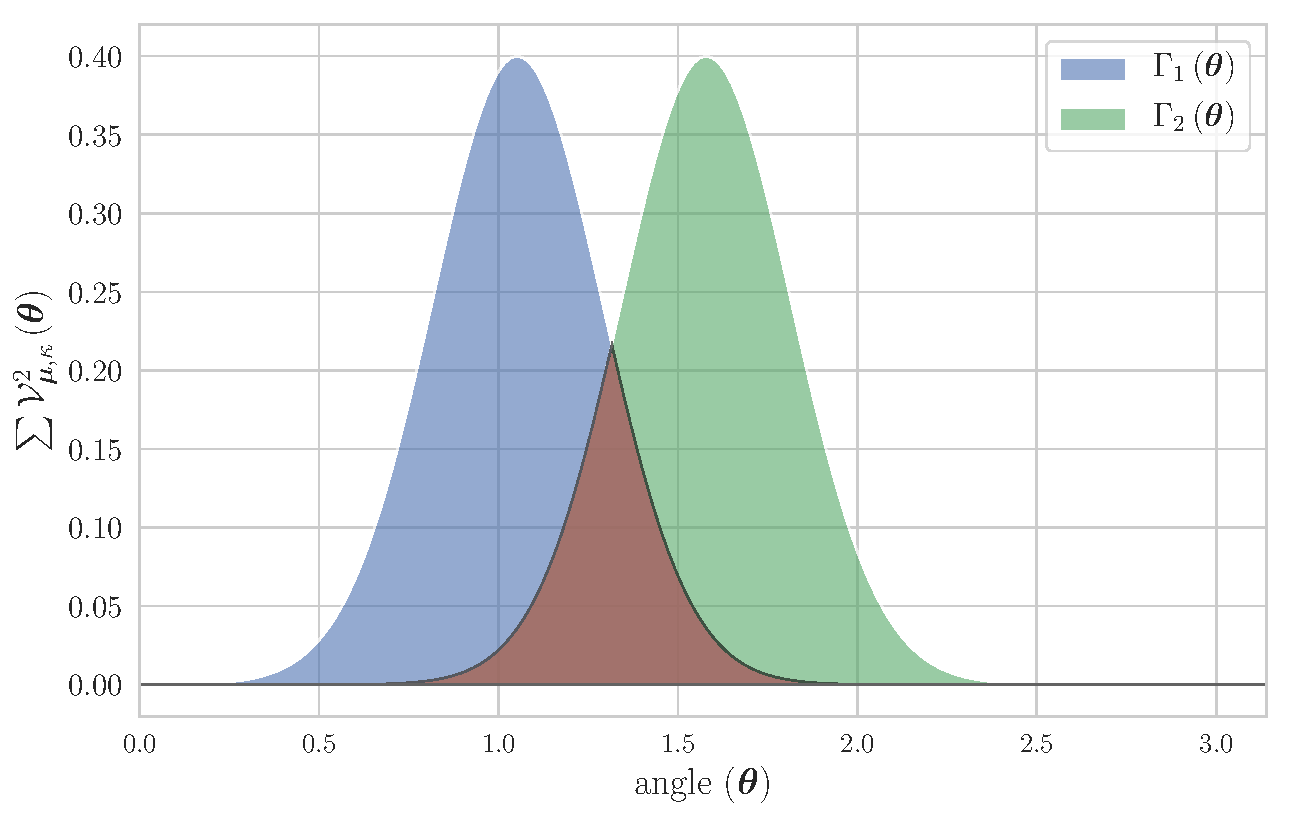
\includegraphics[width=0.8\columnwidth]{angular_deviation}
\par\end{centering}
\centering{}\caption{\vspace{0.05cm}\label{fig: overlap}Two Spatial Von-Mises densities~$\Gamma_{1},\Gamma_{2}$
on the semicircle with respective mean directions~$\mu_{1}=\frac{\pi}{3},\mu_{2}=\frac{\pi}{2}$
and concentration~$\kappa=15$. The red area indicates the overlap
between the spatial densities.}
\end{figure}

In this first round of experiments, we focus on the spatial resolution
of each algorithm, because filtering out components that are spatially
close has many applications, e.g. in audio processing. For this purpose,
we study the filtering performance of mixtures of~$J=2$ real-valued
sources of dimension~$K=2$, so that a direction~$\boldsymbol{\theta}\in\mathcal{S}^{K}$
can be understood as a point on the unit circle.

We take each component~$\boldsymbol{y}_{j}$ as originating mostly
from one direction~$\boldsymbol{\mu}_{j}$, with both components
sharing the same concentration parameter~$\kappa=15$, so that $\Gamma_{j}=\mathcal{V}_{\boldsymbol{\mu}_{j},\kappa}.$
Depending on the choice of the directions~$\boldsymbol{\mu}_{j}$,
this allows us to create some overlap between the~$\Gamma_{j}$'s.
We set a~$0.2$ step-size for $\alpha\in\left[1.2,2\right]$, and
the mean directions~$\boldsymbol{\mu}_{j}$ for the sources are separated
by~$\left\{ 5,15,\dots,85\right\} $ degrees, with~$\boldsymbol{\mu}_{1}$
randomly positioned on the semi-circle. An example is given in Fig.~\ref{fig: overlap}.

Algorithms $\alpha-$SSF and~$\alpha-$CMF were run with partitions
$\Theta$ composed of $P=180$ regions. For each configuration of
the~$\boldsymbol{\mu}_{j}$, the performance of all methods was evaluated
on the filtering of $N=2000$ independent realizations. $100$ different
such experiments were conducted to report the scores.

\begin{figure}
\begin{centering}
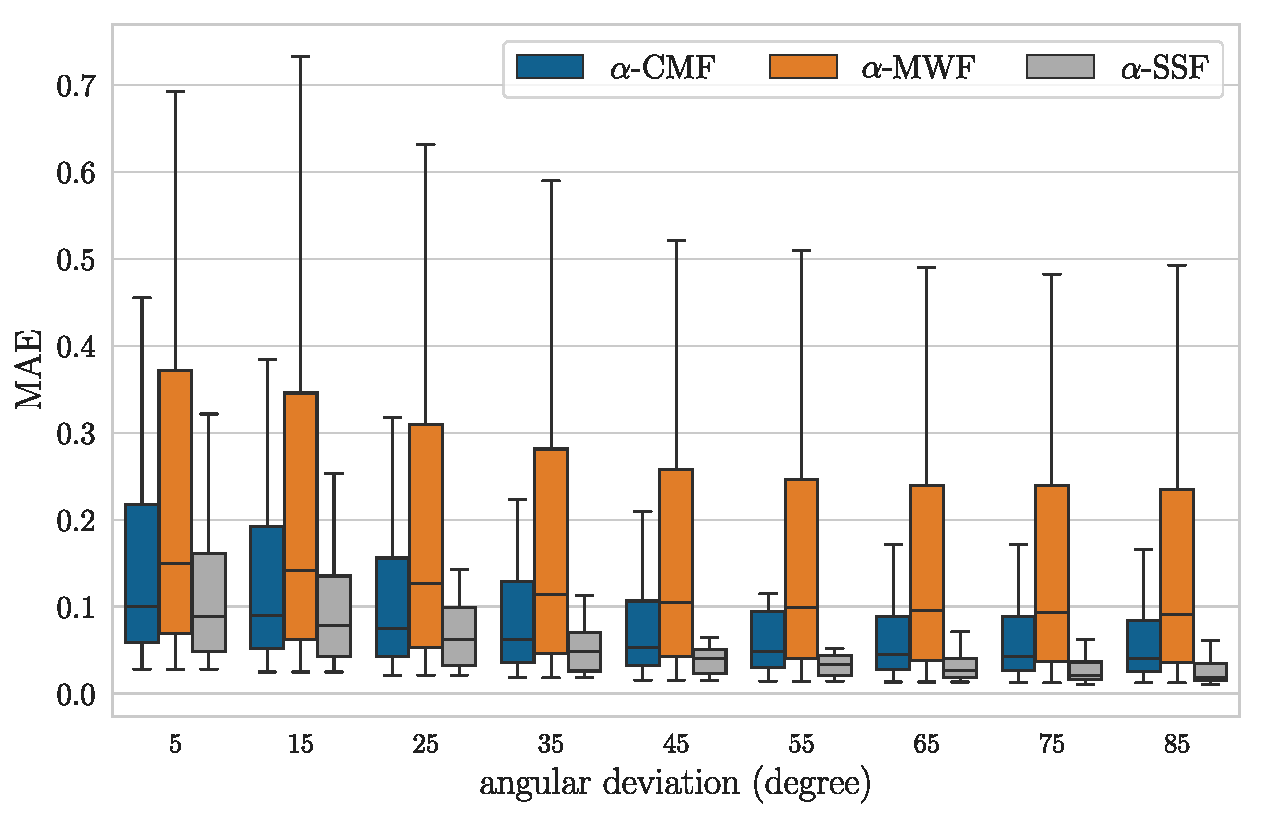
\includegraphics[width=0.8\columnwidth]{experience1-1}
\par\end{centering}
\caption{\label{fig:RMSE-angular_deviation}MAE box plot (lower is better)
of MWF, $\alpha-$CMF and~$\alpha-$SSF methods for several angular
deviations between spatial densities and $\alpha=1.6$. The box plots
shows the minimum and maximum for whiskers, and 75th/25th percentiles
for boxes.}
\end{figure}

\begin{figure}
\begin{centering}
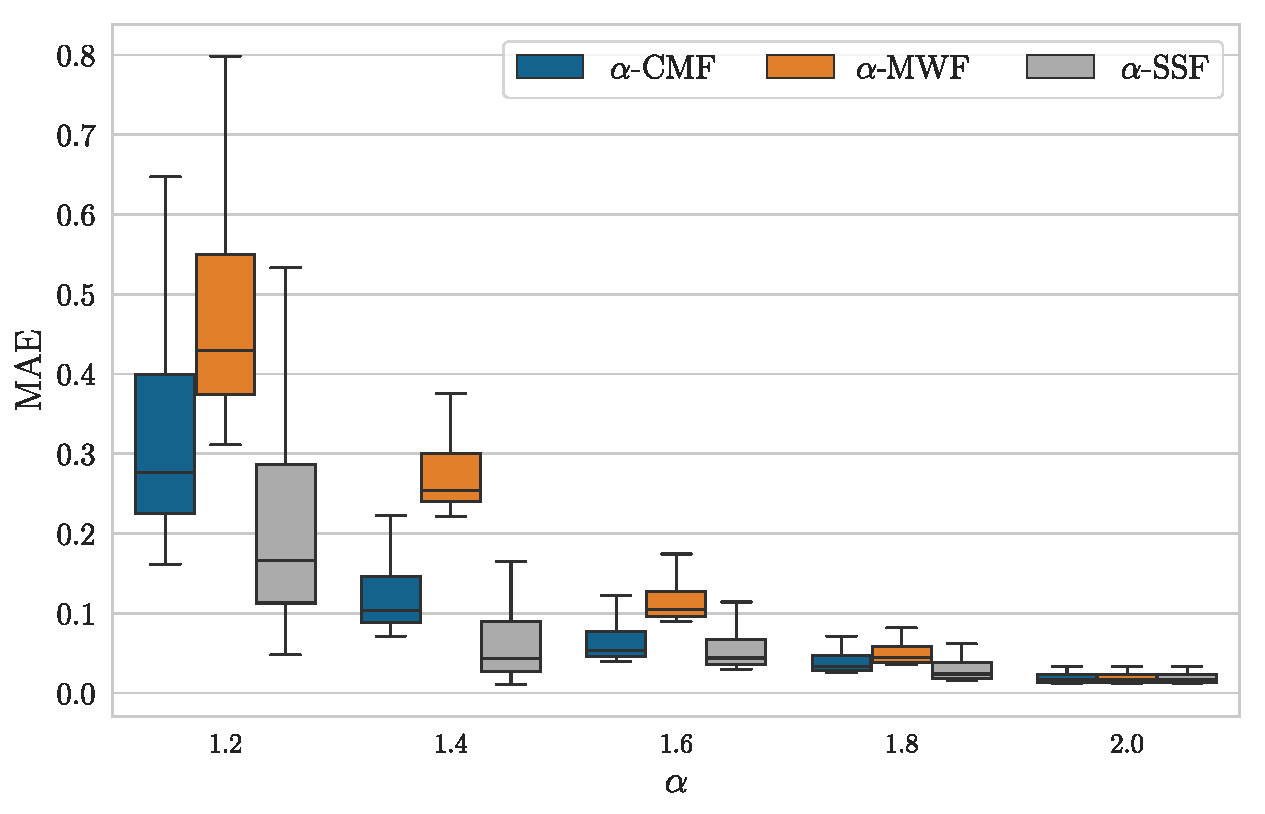
\includegraphics[width=0.8\columnwidth]{experience1-2}
\par\end{centering}
\caption{\label{fig:RMSE-angular_deviation-vs-alpha}MAE performance (lower
is better) as a function of~$\alpha$, for a distance of~$25$ degrees
between the sources.}
\end{figure}

The corresponding MAE~\eqref{eq:MAE} values for $\alpha=1.6$ are
displayed in Fig.~\ref{fig:RMSE-angular_deviation}. As can be seen
on this figure, $\alpha-$SSF globally outperforms the other methods
for all the angular distances between the sources, followed by~$\alpha-$CMF.
While these two methods behave similarly, they both outperform MWF.

In Fig.~\ref{fig:RMSE-angular_deviation-vs-alpha}, we show the evolution
of these scores as a function of $\alpha$, for a fixed deviation
of~$25$ degrees between the sources. As can be seen, smaller values
for~$\alpha$ lead to a degradation of the performance, due to the
extremely heavy tails of the distributions. However, we notice that
all proposed methods remain quite robust. Hence, even MWF, the proposed
approach that exploits the spatial densities~$\Gamma_{j}$ to build
the MWF filters as discussed in Section~\ref{subsec:The-Gaussian-case},
is remarkably effective. In practice, decreasing $P$ often causes
instability for MWF, while increasing $P$ does not significantly
change scores.

\subsection{Performance versus the number of components\label{subsec:Evaluation-complex}}

In this second set of experiments, we evaluate our proposed filtering
methods in the complex case with~$K=2$. Our objective here is to
assess the performance with a varying number $J$ of components to
separate. Hence, for $J\in\left\{ 2,\dots,8\right\} $, $\alpha\in\left[1.2,2\right]$,
and $N=2000$ independent realizations, we run~$100$ independents
experiments, where the spatial densities are VMF distributions with
random parameters $\kappa_{j}$ and $\boldsymbol{\mu}_{j}$.

Regarding the computation of our integrals as in~\eqref{eq:riemann_approx-1}
for this complex case, they were performed with~$P=400$ values for
the partition~$\Theta$.

\begin{figure}
\begin{centering}
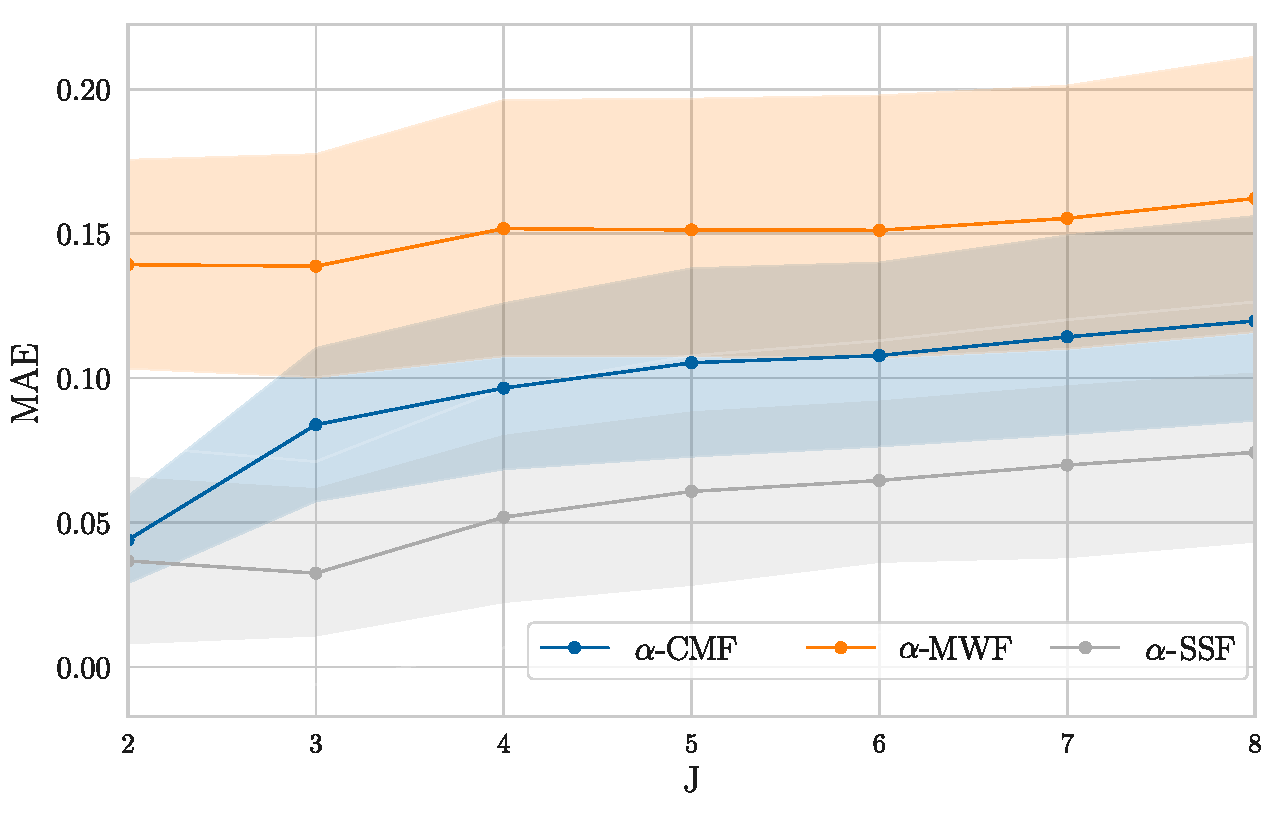
\includegraphics[width=0.8\columnwidth]{experience2}
\par\end{centering}
\caption{MAE averaged over all sources for $\alpha\in\left[1.2,2\right]$.
The solid lines display the median, and the light areas the standard
deviation of each method. \label{fig:RMSE-error-for}}
\end{figure}

The results shown in Fig.~\ref{fig:RMSE-error-for} are in line with
those for~$J=2$ reported above, and suggest that the~$\alpha-$SSF
method globally outperforms the three other methods for all configurations.

\begin{table}[H]
\centering{}{\large{}}%
\begin{tabular}{|c|c|c|c|}
\hline 
 & {\large{}MWF} & {\large{}$\alpha-$CMF} & {\large{}$\alpha-$SSF}\tabularnewline
\hline 
\hline 
{\large{}$J=2$} & \textbf{\large{}0.02} & {\large{}0.18} & {\large{}1.02}\tabularnewline
\hline 
{\large{}$J=3$} & \textbf{\large{}0.02} & {\large{}0.20} & {\large{}1.11}\tabularnewline
\hline 
{\large{}$J=5$} & \textbf{\large{}0.02} & {\large{}0.45} & {\large{}1.12}\tabularnewline
\hline 
{\large{}$J=8$} & \textbf{\large{}0.02} & {\large{}0.65} & {\large{}1.16}\tabularnewline
\hline 
\end{tabular}{\large{}\vspace{0.15cm}}\caption{\label{tab:Elapsed-time}Elapsed time (in sec., lower is better) for
each filtering method.}
\end{table}
Now, we show that this increase of performance comes at the price
of an increased computational cost. Indeed, the computational complexity
of the $\alpha-$SSF method is $\mathcal{O}\left(P^{4}\left(P^{'}\right)^{4}K^{5}N^{3}+JP^{3}K^{2}N\right)$,
where~$P'$ is the number of samples for the discretization of integrals
in~\eqref{eq:numerator} wrt. the Lebesgue measure, while for $\alpha-$CMF
it is $\mathcal{O}\left(IJK^{4}P^{4}N\right)$, where~$I$ denotes
the number of iterations performed in Algorithm~\ref{alg:MASCOT}.
The number $P$ and $P'$ of cells used to sample $\mathcal{S}^{K}$
inherently depends on $K$, and increase exponentially according to
the curse of dimensionality (see~\citet{bellman2013dynamic}). This
explains why evaluations are only performed when $K=2$, and suggests
an important research direction to scale the proposed method to higher
spatial dimensions. In Table~\ref{tab:Elapsed-time}, we report the
average computing time for the different methods to process~$N=2000$
samples, as observed with our Python implementation running on a regular
small laptop computer with an i7-4810MQ CPU and 32 GB of RAM. We observe
that the MWF method is the fastest, followed by $\alpha$-CMF and
by $\alpha$-SSF. Analyzing the methods further, we observe that a
large part of the computing time for $\alpha-$SSF is spent on computing~$\gx\left(\boldsymbol{x},\boldsymbol{\theta}\right)$,
so that separating additional components $J$ doesn't yield a significant
increase in computational load, as for MWF.

\subsection{Filtering spatially scattered sources}

In the preceding sections, we estimated components whose spatial density~$\Gamma_{j}$
was a simple VMF distribution, hence corresponding to only one direction
of arrival~$\mu_{j}$, with some variations brought in by the concentration
parameter~$\kappa_{j}$. We now investigate more diverse spatial
densities, where each (real) source is characterized by several directions
of arrival. This is done by taking each~$\Gamma_{j}$ as a mixture
of $C$ VMF distributions:
\[
\forall j,\:\Gamma_{j}\left(d\boldsymbol{\theta}\right)=\sum_{c}w_{jc}\mathcal{V}_{\boldsymbol{\mu}_{jc},\kappa_{jc}}\left(d\boldsymbol{\theta}\right),
\]
where $\mathcal{V}_{\boldsymbol{\mu}_{jc},\kappa_{jc}}$ is defined
in~\eqref{eq:Von-mises Distribution} and~$w_{jc}\in\left[0,1\right]$
are weight parameters, such that $\forall j,\:\sum_{c}w_{jc}=1$.
Examples of realizations for such models are depicted in Fig.~\ref{fig:Example-of-spatial}
for $K=2$.

We considered~$5$ regularly spaced $\alpha\in\left[1.2,2\right]$
and the separation of $N=2000$ i.i.d. samples from $J=4$ components,
whose spatial densities~$\Gamma_{j}$ are mixtures of $C=2,3,4$
VMF distributions, with parameters $w_{jc}$, $\boldsymbol{\mu}_{jc}$
and $\kappa_{jc}$ drawn randomly anew for each of the $100$ experiments.
The circle is uniformly divided into $P=360$ arcs. 
\begin{figure}[H]
\centering{}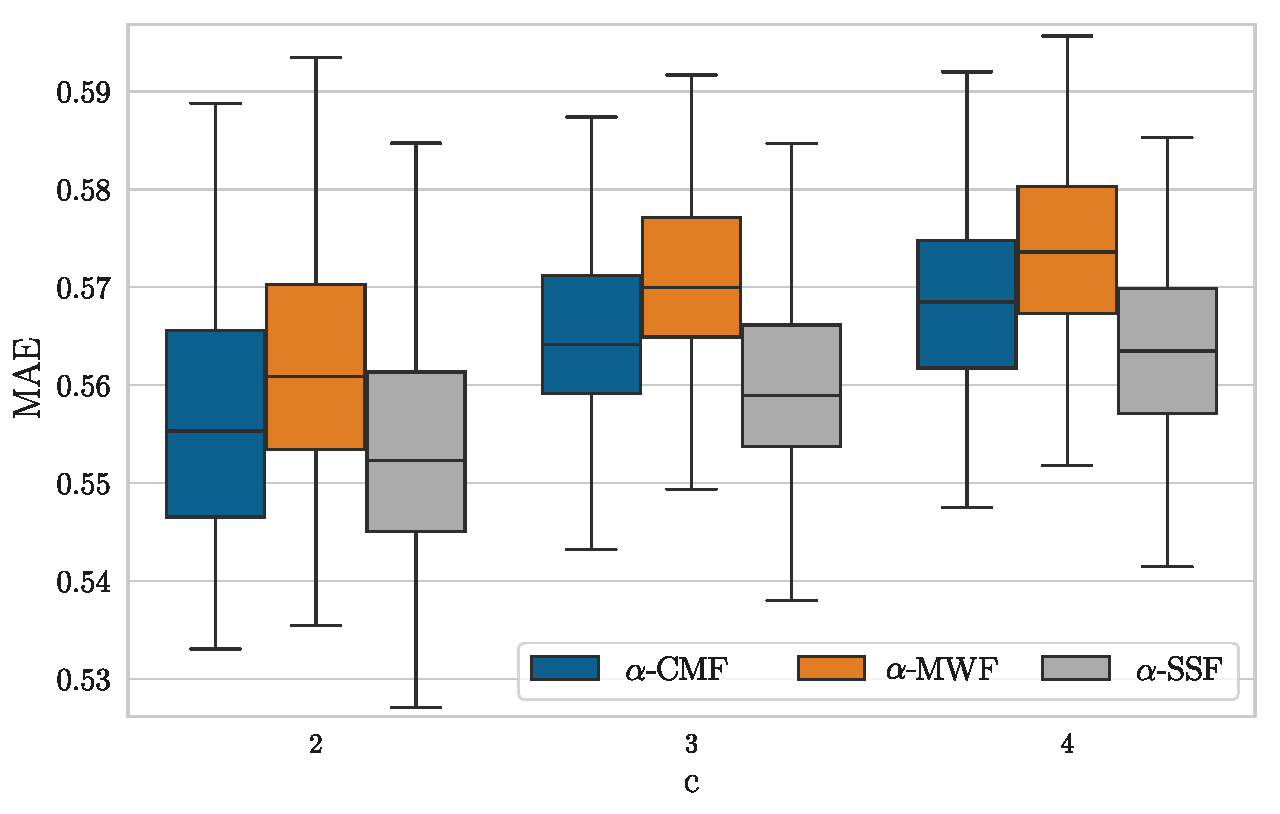
\includegraphics[width=0.8\columnwidth]{experience3}\caption{MAE boxplot for $\alpha=1.4$. \label{fig:experience3}}
\end{figure}

Results for this experiment are depicted in Fig.~\ref{fig:experience3},
giving the MAE as a function of the number $C$ of directions of arrivals
for each component. We see that $\alpha-$SSF slightly outperforms
the other proposed methods and that the performance is overall not
so sensitive to the number of components. We believe that the slight
gain brought in by $\alpha$-SSF can be explained by the fact that
it is a non-linear filter and may hence better handle more sophisticated
spatial models.\vspace{-0.2cm}

\section{Conclusion \& Future works\label{sec:Conclusion-=000026-Future}}

In this paper, we showed how the multivariate symmetric $\alpha$-stable
($S\alpha S$) distribution can be used in filtering applications.

An $S\alpha S$ distribution features remarkably \emph{heavy tails,}
that permit the modeling of signals with very large dynamics. As we
showed, an $S\alpha S$ vector is characterized by a \emph{spatial
density}, that indicates the amount of energy originating from every
direction in space. It hence naturally relaxes the common assumption
of deterministic directions of arrival made for multivariate observations.
One key asset of this model is then to straightforwardly extend to
mixtures of such vectors, owing to the stability property of their
distributions.

Equipped with such a powerful multivariate probabilistic model, we
proposed several filters able to recover $S\alpha S$ vectors from
the observation of their sum. The first one relies on a \emph{spatial
spectrum} decomposition and may be understood as the combination of
a nonlinear beamformer followed by a scalar filter. The second one
enforces \emph{linear} filtering and minimizes the \emph{covariation}
of the difference between estimates and target. As we show, these
filters generalize the classical multivariate Wiener filter to heavy-tailed
signals.

Throughout the paper, we considered the separation of real and complex
$S\alpha S$ vectors. A very straightforward application of these
developments is the filtering of multivariate time series, via their
short-time Fourier transforms. Indeed, this would simply mean generalizing
the recently proposed $\alpha$-harmonizable processes~(\citet{liutkus2015generalized})
to the multivariate case.

A natural route for future work is the combination of such filters
with effective parameter estimation techniques similar to those presented
in~(\citet{fontaine2017EUSIPCO}). All together, they would form
a principled processing pipeline for heavy-tailed and impulsive multivariate
signals. Furthermore, finding a way to proceed to the required integrations
over the hypersphere without a bruteforce partitioning as done here
would allow the use of the proposed method in high-dimensional settings.

\appendix

\section{Proofs\label{sec:Appendix-B}}

\subsection*{1$-$ Proof of spatial representation theorem\label{subsec:Appendix1}}

If $\mathbb{K}=\mathbb{C},$ by substituting in the theorem 6.3.4.
in~(\citet[p. 284]{samoradnitsky1994stable}), the terms:
\begin{align*}
 & \ensuremath{E=\mathcal{S}^{K}},\:\ensuremath{\boldsymbol{x}=\boldsymbol{\theta}},\,\ensuremath{M\left(d\boldsymbol{x}\right)=\mathcal{X}\left(d\boldsymbol{\theta}\right)},\:\ensuremath{m\left(dx\right)=\Gamma_{x}\left(d\boldsymbol{\theta}\right)},\:\ensuremath{d=K},\\
 & \ensuremath{\:j=k,}z_{j}=u_{k},\ensuremath{T=\left[1\ldots K\right]},\:\ensuremath{t_{j}=k},\:\ensuremath{f_{t_{j}}\left(x\right)=x_{t_{j}}=\theta_{k}}
\end{align*}
we get that the chf. of~$\int_{\boldsymbol{\theta}\in\mathcal{S}^{K}}\boldsymbol{\theta}\mathcal{X}\left(d\boldsymbol{\theta}\right)$
is:

{\footnotesize{}
\begin{equation}
\forall\boldsymbol{u}\in\mathbb{C}^{K},\:\mathbb{E}\left[\exp\left(i\Re\left\langle \boldsymbol{u},\int_{\mathcal{S}^{K}}\boldsymbol{\theta}\,\mathcal{X}\left(d\boldsymbol{\theta}\right)\right\rangle \right)\right]=\exp\left(-\int_{\mathcal{S}^{K}}\left|\left\langle \boldsymbol{u},\boldsymbol{\theta}\right\rangle \right|^{\alpha}\Gamma_{x}\left(d\boldsymbol{\theta}\right)\right).\label{eq:stochastic_version}
\end{equation}
}The right side of~\eqref{eq:stochastic_version} is exactly the
chf. of~$\boldsymbol{x}$. This identification achieves the proof
of Theorem~\ref{thm:spatial_representation}.

If $\mathbb{K}=\mathbb{R},$~\eqref{eq:spatial_representation} can
be demonstrated by applying the theorem 3.5.6. in~(\citet[p 131]{samoradnitsky1994stable}).

\subsection*{2$-$ Proof of spatial spectrum estimation\label{subsec:Appendix2}}

\subsubsection*{Proof of Proposition~\ref{prop:spatial_spectrum_form1}}

Let $\forall v\in\mathbb{K},\,c\left(v\right)\triangleq\varphi_{\int_{\boldsymbol{\theta}\in\mathcal{S}^{K}}\psi\left(\boldsymbol{\theta}\right)\mathcal{X}\left(d\boldsymbol{\theta}\right)\mid\boldsymbol{x}}\left(v\right)$.
Note that if the first derivative exists (in the sense of the Wirtinger
derivatives), we have:
\begin{equation}
\mathbb{E}\left[\int_{\boldsymbol{\theta}\in\mathcal{S}^{K}}\psi\left(\boldsymbol{\theta}\right)\mathcal{X}\left(d\boldsymbol{\theta}\right)\mid\boldsymbol{x}\right]=-i\frac{dc}{dv^{\star}}\left(v=0\right).\label{eq:conditionnal_expectation}
\end{equation}

\begin{comment}
Attention, $\nu$ �tant un param�tre complexe, il faut pr�ciser dans
quel sens la d�riv�e par rapport � $\nu$ est d�finie (sachant que
la fonction $c$ n'est clairement pas analytique par rapport � $\nu$).
\end{comment}

In order to find a suitable form of~$c$, we start by calculating
the joint chf. of~$\int_{\boldsymbol{\theta}\in\mathcal{S}^{K}}\psi\left(\boldsymbol{\theta}\right)\mathcal{X}\left(d\boldsymbol{\theta}\right)$
and~$\boldsymbol{x},\,\forall v\in\mathbb{K},\,\forall\boldsymbol{u}\in\mathbb{K}^{K}$:
\begin{align*}
\varphi_{\left(\int_{\boldsymbol{\theta}\in\mathcal{S}^{K}}\psi\left(\boldsymbol{\theta}\right)\mathcal{X}\left(d\boldsymbol{\theta}\right),\boldsymbol{x}\right)}\left(v,\boldsymbol{u}\right) & \triangleq\mathbb{E}\left[e^{i\Re\left(v^{\ast}\int_{\boldsymbol{\theta}\in\mathcal{S}^{K}}\psi\left(\boldsymbol{\theta}\right)\,\mathcal{X}\left(d\boldsymbol{\theta}\right)+\left\langle \boldsymbol{u},\boldsymbol{x}\right\rangle \right)}\right]\\
 & =\mathbb{E}\left[e^{i\Re\left(\int_{\boldsymbol{\theta}\in\mathcal{S}^{K}}\left(v^{\ast}\psi\left(\boldsymbol{\theta}\right)+\left\langle \boldsymbol{u},\boldsymbol{\theta}\right\rangle \right)\:\mathcal{X}\left(d\boldsymbol{\theta}\right)\right)}\right]\\
 & =\varphi_{\int_{\boldsymbol{\theta}\in\mathcal{S}^{K}}\left(v^{\ast}\psi\left(\boldsymbol{\theta}\right)+\langle\boldsymbol{u},\boldsymbol{\theta}\rangle\right)\:\mathcal{X}\left(d\boldsymbol{\theta}\right)}\left(1\right)\\
 & =e^{-\int_{\boldsymbol{\theta}\in\mathcal{S}^{K}}\left|v^{\ast}\psi\left(\boldsymbol{\theta}\right)+\left\langle \boldsymbol{u},\boldsymbol{\theta}\right\rangle \right|{}^{\alpha}\:\Gamma_{\boldsymbol{x}}\left(d\boldsymbol{\theta}\right)},
\end{align*}
where the last equality holds because

\[
\begin{array}{c}
\int_{\boldsymbol{\theta}\in\mathcal{S}^{K}}\left(v^{\ast}\psi\left(\boldsymbol{\theta}\right)+\left\langle \boldsymbol{u},\boldsymbol{\theta}\right\rangle \right)\:\mathcal{X}\left(d\boldsymbol{\theta}\right)\\
\sim S\alpha S_{c}^{K}\left(\int_{\boldsymbol{\theta}\in\mathcal{S}^{K}}\left|v^{\ast}\psi(\boldsymbol{\theta})+\langle\boldsymbol{u},\boldsymbol{\theta}\rangle\right|{}^{\alpha}\:\Gamma_{\boldsymbol{x}}\left(d\boldsymbol{\theta}\right)\right).
\end{array}
\]
Thus, $c$ has the following form:~$\forall v\in\mathbb{K}$,

\begin{align}
c(v) & =\frac{\int_{\boldsymbol{u}\in\mathbb{K}^{K}}\varphi_{\int_{\boldsymbol{\theta}\in\mathcal{S}^{K}}\psi\left(\boldsymbol{\theta}\right)\mathcal{X}\left(d\boldsymbol{\theta}\right),\boldsymbol{x}}\left(v,\boldsymbol{u}\right)e^{-i\Re\left(\left\langle \boldsymbol{u},\boldsymbol{x}\right\rangle \right)}d\boldsymbol{u}}{\int_{\boldsymbol{u}\in\mathbb{K}^{K}}\varphi_{\boldsymbol{x}}\left(\boldsymbol{u}\right)e^{-i\Re\left(\left\langle \boldsymbol{u},\boldsymbol{x}\right\rangle \right)}d\boldsymbol{u}}\nonumber \\
 & =\frac{\int_{\boldsymbol{u}\in\mathbb{K}^{K}}e^{-\int_{\boldsymbol{\theta}\in\mathcal{S}^{K}}\left|v^{\ast}\psi(\boldsymbol{\theta})+\langle\boldsymbol{u},\boldsymbol{\theta}\rangle\right|{}^{\alpha}\:\Gamma_{\boldsymbol{x}}\left(d\boldsymbol{\theta}\right)}e^{-i\Re\left(\left\langle \boldsymbol{u},\boldsymbol{x}\right\rangle \right)}d\boldsymbol{u}}{\int_{\boldsymbol{u}\in\mathbb{K}^{K}}\varphi_{\boldsymbol{x}}\left(\boldsymbol{u}\right)e^{-i\Re\left(\left\langle \boldsymbol{u},\boldsymbol{x}\right\rangle \right)}d\boldsymbol{u}}.\label{eq:chf_form_spatial_spectrum}
\end{align}
The existence of~$\frac{dc}{dv^{\star}}\left(v=0\right)$ is because
\[
\nu\mapsto\int_{\boldsymbol{u}\in\mathbb{K}^{K}}\varphi_{\int_{\boldsymbol{\theta}\in\mathcal{S}^{K}}\psi\left(\boldsymbol{\theta}\right)\mathcal{X}\left(d\boldsymbol{\theta}\right),\boldsymbol{x}}\left(v,\boldsymbol{u}\right)e^{-i\Re\left(\left\langle \boldsymbol{u},\boldsymbol{x}\right\rangle \right)}d\boldsymbol{u}
\]
 is the Fourier transform of a characteristic function whose first
derivative exists because~$\alpha>1$~(if a random vector admits
a $1^{st}$ order moment, then its characteristic function is continuously
differentiable at zero). Consequently, by using the differentiation
under the integral sign theorem (the domination is induced by the
fact that a chf. is bounded by~$1$) and by combining~\eqref{eq:conditionnal_expectation}
and~\eqref{eq:chf_form_spatial_spectrum} we obtain:

\begin{equation}
\begin{array}{cc}
 & \mathbb{E}\left[\int_{\boldsymbol{\theta}\in\mathcal{S}^{K}}\psi\left(\boldsymbol{\theta}\right)\mathcal{X}\left(d\boldsymbol{\theta}\right)\mid\boldsymbol{x}\right]\\
= & \frac{\alpha i\int_{\boldsymbol{u}\in\mathbb{K}^{K}}\left(\int_{\boldsymbol{\theta}\in\mathcal{S}^{K}}\psi\left(\boldsymbol{\theta}\right)\left\langle \boldsymbol{\theta},\boldsymbol{u}\right\rangle {}^{\left\langle \alpha-1\right\rangle }\Gamma_{\boldsymbol{x}}\left(d\boldsymbol{\theta}\right)\right)\varphi_{\boldsymbol{x}}\left(\boldsymbol{u}\right)e^{-i\Re\left(\left\langle \boldsymbol{u},\boldsymbol{x}\right\rangle \right)}du}{\int_{\boldsymbol{u}\in\mathbb{K}^{K}}\varphi_{\boldsymbol{x}}\left(\boldsymbol{u}\right)e^{-i\Re\left(\left\langle \boldsymbol{u},\boldsymbol{x}\right\rangle \right)}d\boldsymbol{u}}\\
= & \int_{\boldsymbol{\theta}\in\mathcal{S}^{K}}\psi\left(\boldsymbol{\theta}\right)\left[\frac{\alpha i\int_{\boldsymbol{u}\in\mathbb{K}^{K}}\left\langle \boldsymbol{\theta},\boldsymbol{u}\right\rangle {}^{\left\langle \alpha-1\right\rangle }\varphi_{\boldsymbol{x}}\left(\boldsymbol{u}\right)\,e^{-i\Re\left(\left\langle \boldsymbol{u},\boldsymbol{x}\right\rangle \right)}d\boldsymbol{u}}{\int_{\boldsymbol{u}\in\mathbb{K}^{K}}\varphi_{\boldsymbol{x}}\left(\boldsymbol{u}\right)\,e^{-i\Re\left(\left\langle \boldsymbol{u},\boldsymbol{x}\right\rangle \right)}d\boldsymbol{u}}\right]\Gamma_{\boldsymbol{x}}\left(d\boldsymbol{\theta}\right)\\
= & \int_{\boldsymbol{\theta}\in\mathcal{S}^{K}}\psi\left(\boldsymbol{\theta}\right)\gx\left(\boldsymbol{x},\boldsymbol{\theta}\right)\Gamma_{\boldsymbol{x}}\left(d\boldsymbol{\theta}\right).
\end{array}\label{eq:end_calculation_cond_exp}
\end{equation}
where we have used~\eqref{eq:estimation_g_x_theta}. Equation~\eqref{eq:estimator_form}
is obtained by identifying~\eqref{eq:end_calculation_cond_exp} with~\eqref{eq:estimator_criterion}
for any continuous function $\psi\left(\boldsymbol{\theta}\right)$.

\vspace{0.5cm}

\subsubsection*{Proof of Proposition~\ref{prop:spatial_spectrum_form1} about continuity}

$\forall\boldsymbol{u}\in\mathbb{K}^{K},\:\boldsymbol{\theta}\mapsto h\left(\boldsymbol{\theta},\boldsymbol{u}\right)=\left\langle \boldsymbol{\theta},\boldsymbol{u}\right\rangle ^{\left\langle \alpha-1\right\rangle }\varphi_{\boldsymbol{x}}\left(\boldsymbol{u}\right)e^{-i\Re(\left\langle \boldsymbol{u},\boldsymbol{x}\right\rangle )}$
is a continuous function. Moreover, the probability density function
(pdf.) of an~$S\alpha S_{c}$ (non-degenerated) distribution is infinitely
continuous. As a result, the characteristic function~$\varphi_{\boldsymbol{x}}\left(\boldsymbol{u}\right)$
for all \textbf{$\boldsymbol{u}\in\mathbb{K}^{K}$}(which is the Fourier
transform of a pdf.) decreases faster than any power of $\left\Vert u\right\Vert $
(where~$\left\Vert .\right\Vert $ is any norm on~$\mathbb{K}^{K}$).
In particular, $\boldsymbol{u}\mapsto f\left(\boldsymbol{u}\right)=\left\Vert \boldsymbol{u}\right\Vert ^{\alpha-1}\left|\varphi_{x}\left(\boldsymbol{u}\right)\right|$
is integrable. Besides, $\forall\boldsymbol{\theta}\in\mathcal{S}^{K},$
$\left|\left\langle \boldsymbol{\theta},\boldsymbol{u}\right\rangle ^{\left\langle \alpha-1\right\rangle }\right|\leq\left\Vert \boldsymbol{u}\right\Vert ^{\alpha-1}$
and $\forall\boldsymbol{u}\in\mathbb{K}^{K},\,\left|h\left(\boldsymbol{\theta},\boldsymbol{u}\right)\right|\leq f\left(\boldsymbol{u}\right)$.
By applying the theorem of continuity under the integral sign, we
conclude that~$\gx\left(\boldsymbol{x},\boldsymbol{\theta}\right)$
is a continuous function of~$\boldsymbol{\theta}$.

\subsubsection*{Proof of Proposition~\ref{prop:numerator_calculation}}

We consider the numerator~$N\left(\boldsymbol{x},\boldsymbol{\theta}\right)$
of~$\gx\left(\boldsymbol{x},\boldsymbol{\theta}\right)$ in \eqref{eq:N}
and apply the change of variables~$\boldsymbol{u}\triangleq r\boldsymbol{\theta}'\in\mathbb{K}^{K}$
where~$r\in\mathbb{R}^{+}$and $\boldsymbol{\theta}'\in\mathcal{S}^{K}$,
which is such that $d\boldsymbol{u}=r^{\beta K-1}drd\boldsymbol{\theta}'$.
Then we get:

{\footnotesize{}
\begin{multline*}
N\left(\boldsymbol{x},\boldsymbol{\theta}\right)=i\int_{\boldsymbol{\theta}'\in\mathcal{S}^{K}}\left\langle \boldsymbol{\theta},\boldsymbol{\theta'}\right\rangle {}^{\left\langle \alpha-1\right\rangle }\\
\qquad\qquad\qquad\left(\int_{r\in\mathbb{R}_{+}}\left(\alpha r^{\alpha-1}e^{-r^{\alpha}I_{\boldsymbol{x}}\left(\boldsymbol{\theta'}\right)}\right)\left(r^{\beta K-1}e^{-ir\Re\left(\left\langle \boldsymbol{\theta'},\boldsymbol{x}\right\rangle \right)}\right)dr\right)d\boldsymbol{\theta'}.
\end{multline*}
}Applying an integration by parts to{\footnotesize{} $\int_{r\in\mathbb{R}_{+}}\left(\alpha r^{\alpha-1}e^{-r^{\alpha}I_{\boldsymbol{x}}\left(\boldsymbol{\theta'}\right)}\right)\left(r^{\beta K-1}e^{-ir\Re\left(\left\langle \boldsymbol{\theta'},\boldsymbol{x}\right\rangle \right)}\right)dr$}
yields:

\[
N\left(\boldsymbol{x},\boldsymbol{\theta}\right)=A\left(\boldsymbol{\theta},\boldsymbol{x}\right)+\left(\beta K-1\right)iB\left(\boldsymbol{\theta},\boldsymbol{x}\right)
\]
where{\footnotesize{}
\begin{align*}
A\left(\boldsymbol{\theta},\boldsymbol{x}\right) & =\int_{\boldsymbol{\theta}'\in\mathcal{S}^{K}}\frac{\left\langle \boldsymbol{\theta},\boldsymbol{\theta'}\right\rangle {}^{\left\langle \alpha-1\right\rangle }\Re\left(\left\langle \boldsymbol{\theta'},\boldsymbol{x}\right\rangle \right)}{I_{\boldsymbol{x}}\left(\boldsymbol{\theta'}\right)}\\
 & \qquad\qquad\qquad\qquad\left(\int_{r\in\mathbb{R}_{+}}r^{\beta K-1}e^{-r^{\alpha}I_{\boldsymbol{x}}\left(\boldsymbol{\theta'}\right)}e^{-ir\Re\left(\left\langle \boldsymbol{\theta'},\boldsymbol{x}\right\rangle \right)}dr\right)d\boldsymbol{\theta'}\\
B\left(\boldsymbol{\theta},\boldsymbol{x}\right) & =\int_{\boldsymbol{\theta}'\in\mathcal{S}^{K}}\frac{\left\langle \boldsymbol{\theta},\boldsymbol{\theta'}\right\rangle {}^{\left\langle \alpha-1\right\rangle }}{I_{\boldsymbol{x}}\left(\boldsymbol{\theta'}\right)}\\
 & \qquad\qquad\qquad\qquad\left(\int_{r\in\mathbb{R}_{+}}r^{\beta K-2}e^{-r^{\alpha}I_{\boldsymbol{x}}\left(\boldsymbol{\theta'}\right)}e^{-ir\Re\left(\left\langle \boldsymbol{\theta'},\boldsymbol{x}\right\rangle \right)}dr\right)d\boldsymbol{\theta'}.
\end{align*}
}By developing the complex exponential as a power series and by applying
the identity~$\int_{0}^{+\infty}x^{n}e^{-ax^{b}}dx=\frac{1}{b}a^{-\frac{n+1}{b}}f_{\Gamma}\left(\frac{n+1}{b}\right)$
to both integrals~$A\left(\boldsymbol{\theta},\boldsymbol{x}\right)$
and $B\left(\boldsymbol{\theta},\boldsymbol{x}\right)$, we get:

{\scriptsize{}
\begin{align}
A\left(\boldsymbol{\theta},\boldsymbol{x}\right) & =\tfrac{1}{\alpha}\int_{\boldsymbol{\theta}'\in\mathcal{S}^{K}}\sum_{n=0}^{+\infty}\tfrac{\left(-i\right){}^{n}f_{\Gamma}\left(\frac{n+\beta K}{\alpha}\right)}{n!}\tfrac{\langle\boldsymbol{\theta},\boldsymbol{\theta'}\rangle^{<\alpha-1>}\frac{1}{2^{n+1}}\mathcal{B}_{n+1}\left(\langle\boldsymbol{\theta'},\boldsymbol{x}\rangle,\langle\boldsymbol{x},\boldsymbol{\theta'}\rangle\right)}{I_{\boldsymbol{x}}(\boldsymbol{\theta'})^{\frac{n+\beta K+\alpha}{\alpha}}}d\boldsymbol{\theta'}\label{eq:A}\\
B\left(\boldsymbol{\theta},\boldsymbol{x}\right) & =\tfrac{1}{\alpha}\int_{\boldsymbol{\theta}'\in\mathcal{S}^{K}}\sum_{n=0}^{+\infty}\tfrac{(-i)^{n}f_{\Gamma}\left(\frac{n+\beta K-1}{\alpha}\right)}{n!}\tfrac{\left\langle \boldsymbol{\theta},\boldsymbol{\theta'}\right\rangle {}^{\left\langle \alpha-1\right\rangle }\frac{1}{2^{n}}\mathcal{B}_{n}\left(\langle\boldsymbol{\theta'},\boldsymbol{x}\rangle,\langle\boldsymbol{x},\boldsymbol{\theta'}\rangle\right)}{I_{\boldsymbol{x}}\left(\boldsymbol{\theta'}\right){}^{\frac{n+\beta K-1+\alpha}{\alpha}}}d\boldsymbol{\theta'}.\label{eq:B}
\end{align}
}where $\mathcal{B}_{n}\left(u,v\right)=\left(u+v\right){}^{n}=\sum_{k=0}^{n}\dbinom{n}{k}u^{n}v^{n-k}$.
Finally, we remark from~\eqref{eq:N} that $N\left(z\boldsymbol{x},\boldsymbol{\theta}\right)=zN\left(\boldsymbol{x},\boldsymbol{\theta}\right),\forall z\in\mathcal{S}_{\mathbb{K}}^{1}$,
which shows that in~\eqref{eq:A}, all odd values of $n$, and all
values of $k$ different from $\frac{n}{2}+1$, can be discarded (the
corresponding terms vanish when integrated). In the same way, in~\eqref{eq:B},
all even values of $n$, and all values of $k$ different from $\frac{n+1}{2}$,
can be discarded, which finally leads to~\eqref{eq:numerator} and~\eqref{eq:eta}.
Equation~\eqref{eq:eta} defines a power series with an infinite
radius of convergence when~$\alpha>1$, which is smooth and independent
the mixing model.

The estimate of~$\boldsymbol{x}\to D\left(\boldsymbol{x}\right)$
is obtained by noting that:

\[
\boldsymbol{x}=\int_{\boldsymbol{\theta}\in\mathcal{S}^{K}}\boldsymbol{\theta}\gx\left(\boldsymbol{x},\boldsymbol{\theta}\right)\Gamma_{x}\left(d\boldsymbol{\theta}\right)=\int_{\boldsymbol{\theta}\in\mathcal{S}^{K}}\boldsymbol{\theta}\frac{N\left(\boldsymbol{x},\boldsymbol{\theta}\right)}{D\left(\boldsymbol{x}\right)}\Gamma_{\boldsymbol{x}}\left(d\boldsymbol{\theta}\right).
\]

\vspace{0.5cm}

\subsubsection*{Proof of Theorem~\ref{thm:source_reconstruction}}

We first determine the joint chf. of~$\boldsymbol{y}_{j}$ and~$\boldsymbol{x}$:~$\forall\boldsymbol{v},\boldsymbol{u}\in\mathbb{K}^{K}$,
\begin{align*}
\varphi_{\left(\boldsymbol{y}_{j},\boldsymbol{x}\right)}\left(\boldsymbol{v},\boldsymbol{u}\right) & \triangleq\mathbb{E}\left[e^{i\Re\left(\left\langle \boldsymbol{v},\boldsymbol{y}_{j}\right\rangle +\left\langle \boldsymbol{u},\boldsymbol{x}\right\rangle \right)}\right]\\
 & =\mathbb{E}\left[e^{i\Re\left(\left\langle \boldsymbol{v}+\boldsymbol{u},\boldsymbol{y}_{j}\right\rangle +\sum_{j'\neq j}\left\langle \boldsymbol{u},\boldsymbol{y}_{j'}\right\rangle \right)}\right]\\
 & =\varphi_{\boldsymbol{y}_{j}}\left(\boldsymbol{v}+\boldsymbol{u}\right)\prod_{j'\neq j}\varphi_{\boldsymbol{y}_{j'}}\left(\boldsymbol{u}\right)\\
 & =e^{-\int_{\boldsymbol{\theta}\in\mathcal{S}^{K}}\left|\left\langle \boldsymbol{v}+\boldsymbol{u},\boldsymbol{\theta}\right\rangle \right|{}^{\alpha}\Gamma_{j}\left(d\boldsymbol{\theta}\right)-\sum_{j'\neq j}\int_{\boldsymbol{\theta}\in\mathcal{S}^{K}}\left|\left\langle \boldsymbol{u},\boldsymbol{\theta}\right\rangle \right|{}^{\alpha}\Gamma_{j'}\left(d\boldsymbol{\theta}\right)},
\end{align*}
which permits us to deduce the chf. of~$\boldsymbol{y}_{j}$ given~$\boldsymbol{x},$~$\forall\boldsymbol{v}\in\mathbb{K}^{K}:$
\[
\begin{array}{c}
\varphi_{\boldsymbol{y}_{j}|\boldsymbol{x}}\left(\boldsymbol{v}\right)=\frac{\int_{\boldsymbol{u}\in\mathbb{K}^{K}}e^{-\int_{\boldsymbol{\theta}\in\mathcal{S}^{K}}\left|\left\langle \boldsymbol{v}+\boldsymbol{u},\boldsymbol{\theta}\right\rangle \right|{}^{\alpha}\Gamma_{j}\left(d\boldsymbol{\theta}\right)-\sum_{j'\neq j}\int_{\boldsymbol{\theta}\in\mathcal{S}^{K}}\left|\left\langle \boldsymbol{u},\boldsymbol{\theta}\right\rangle \right|{}^{\alpha}\Gamma_{j'}\left(d\boldsymbol{\theta}\right)}e^{-i\Re\left(\left\langle \boldsymbol{u},\boldsymbol{x}\right\rangle \right)}d\boldsymbol{u}}{\int_{\boldsymbol{u}\in\mathbb{K}^{K}}\varphi_{\boldsymbol{x}}\left(\boldsymbol{u}\right)e^{-i\Re\left(\left\langle \boldsymbol{u},\boldsymbol{x}\right\rangle \right)}d\boldsymbol{u}}.\\
\\
\end{array}
\]
The proof of the existence of~$\nabla_{\boldsymbol{v}^{\star}}\varphi_{\boldsymbol{y}_{j}\mid\boldsymbol{x}}$
is exactly the same as in Proposition~\ref{prop:spatial_spectrum_form1}.
Thus, we get:

{\footnotesize{}
\begin{align*}
\mathbb{E}\left[\boldsymbol{y}_{j}\mid\boldsymbol{x}\right] & =-i\nabla_{\boldsymbol{v}^{\star}}\varphi_{\boldsymbol{y}_{j}|\boldsymbol{x}}\left(\boldsymbol{v}=\boldsymbol{0}\right)\\
 & =\int_{\boldsymbol{\theta}\in\mathcal{S}^{K}}\boldsymbol{\theta}\left[\frac{\alpha i\int_{\boldsymbol{u}\in\mathbb{K}^{K}}\left\langle \boldsymbol{u},\boldsymbol{\theta}\right\rangle {}^{\left\langle \alpha-1\right\rangle }\varphi_{\boldsymbol{x}}\left(\boldsymbol{u}\right)\,e^{-i\Re\left(\left\langle \boldsymbol{u},\boldsymbol{x}\right\rangle \right)}d\boldsymbol{u}}{\int_{\boldsymbol{u}\in\mathbb{K}^{K}}\varphi_{\boldsymbol{x}}\left(\boldsymbol{u}\right)\,e^{-i\Re\left(\left\langle \boldsymbol{u},\boldsymbol{x}\right\rangle \right)}d\boldsymbol{u}}\right]\Gamma_{j}\left(d\boldsymbol{\theta}\right)\\
 & =\int_{\boldsymbol{\theta}\in\mathcal{S}^{K}}\boldsymbol{\theta}\,\gx\left(\boldsymbol{x},\boldsymbol{\theta}\right)\Gamma_{j}\left(d\boldsymbol{\theta}\right),
\end{align*}
} which completes the proof.

\section*{\textemdash \textemdash \textemdash \textemdash \textemdash \textendash{}}

\bibliographystyle{elsarticle-harv}
\addcontentsline{toc}{section}{\refname}\bibliography{alpha_theory}

\end{document}
